\section{Hierarchical aggregations}

\subsection{Theoretical framework} To facilitate the integration of additional input Measures into
the report card scores (such as additional Physical or Chemical), or even additional Sub-indicators
(such as sediment metals, aquaculture yields etc), we can defined a hierarchical structure in which
Measures (such as Chlorpohyll-a, NOx, sediment aluminum and yield etc) are nested within appropriate
Sub-indicators.  In turn, these Sub-indicators are nested within Indicators.

By progressively abstracting away the details of the Measures and Sub-indicators, a more focused
narrative can be formulated around each level of the hierarchy. For example, when discussing the
current state (and trend in state) of the Water Quality Indicator, rather than needing to discuss
each individual constituent of Water Quality, high-level Grades are available on which to base
high-level interpretations.  More detailed explorations are thence revealed as required by exploring
the Grades at progressively finer scales of the hierarchy.  Moreover, the hierarchical structure
offers great redundancy and thus flexibility to add, remove and exchange individual measures.
   
Similar arguments can be made for a spatial hierarchy in which Sites are nested within Zones which
in turn are nested within the Whole GBR.
    
The purpose of aggregation is to combine together multiple items of data.  For Nesp 3.2.5, the
report card is informed by a triple hierarchical data structure in which Daily observations are
nested within Seasonal and Annual aggregates, Measures are nested within Sub-indicators which are
nested in Indicators and Sites are nested within Zones (see Figure \ref{fig:hierarchies}).


\begin{figure}[h]
\begin{center}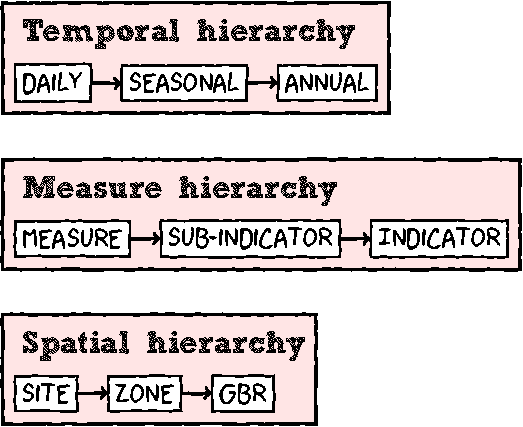
\includegraphics[width=0.5\linewidth]{figures/Diagrams/hierarchies.pdf}}\end{center}
\caption{Temporal, measure and spatial aggregation hierarchy}\label{fig:hierarchies}
\end{figure}


Although the triple hierarchy (temporal, Spatial and Measurement), does offer
substantial redundancy and power advantages, it also introduce the
complexity of how to combine the hierarchies into a single hierarchical
aggregation schedule. Table \ref{tab:complexity} (a fabricated example),
illustrates this complexity for aggregating across Spatial and Measure
scales when data availability differs. This simple example demonstrates
how different aggregation schedules can result in different Zone Indicator scores:



\begin{itemize}
\itemsep1pt\parskip0pt\parsep0pt
\item calculating Zone 1 Indicator Score as the average of the Site level Water Quality Scores
prioritizes that the Zone 1 Indicator Score should reflect the average of the Water Quality
Indicator Scores for the Site. This routine will bias the resulting Zone 1 Water Quality Indicator
Score towards Sub-indicators represented in more Sites.  The current MMP sampling design is
unbalanced (some Zones have more Sites than others and not all Measures are observed in all Sites),
and there is no guarantee that the design will be maintained over time. If for example, Chemical
Measures were not available for certain Zones, then the Whole GBR Water Quality Indicator Score will
be biased towards Water Clarity Sub-indicators.
\item calculating Zone 1 Water Quality Indicator Score as the average of the Zone 1 level
Sub-indicator Scores prioritizes equal contributions of Sub-indicators to the Indicator Score at the
expense of being able to relate Zone 1 Scores to the corresponding Site Scores.
\end{itemize}

The above becomes even more complex when the temporal dimension is include..

\begin{table}[htb]
\centering\scriptsize\scriptsize
\begin{minipage}{0.57\linewidth}
\caption{Fabricated illustration of the discrepancies between total means (i.e. Zone 1 Indicator Score) generated from row means (Site Sub-indicator Scores) and column means (Zone 1 Sub-indicator Scores).}\label{tab:complexity}
\scriptsize
\begin{tabular}{l|cc||c}
\toprule
&\multicolumn{2}{c}{\textbf{Sub-indicators}}&\\
\cmidrule(rl){2-3}
\textbf{Site}&\textbf{Water Clarity}&\textbf{Nutrients}&\textbf{Indicator}\\
\midrule
1&5&2&3.50\\
2&6&&6.00\\
3&6&4&5.00\\
\midrule
Zone 1&5.67&3.00&X\\
\bottomrule
\end{tabular}\\
If X (mean) is calculated from the three row means = 4.83\\
If X (mean) is calculated from the two column means = 4.33
\end{minipage}
\end{table}



An additional complication is how the different hierarchies integrate together.  Specifically, what
level of data should be aggregated first and at what point do the aggregations of one hierarchy feed
into other hierarchies. For example, should observations first be aggregated from Daily to Seasonal
or Annual, then aggregated from Site level to Zone level and then finally aggregated from Measure to
Indicator?  Some possible configurations are presented in Figure \ref{fig:hier}.


\begin{landscape}
\begin{figure}[h]
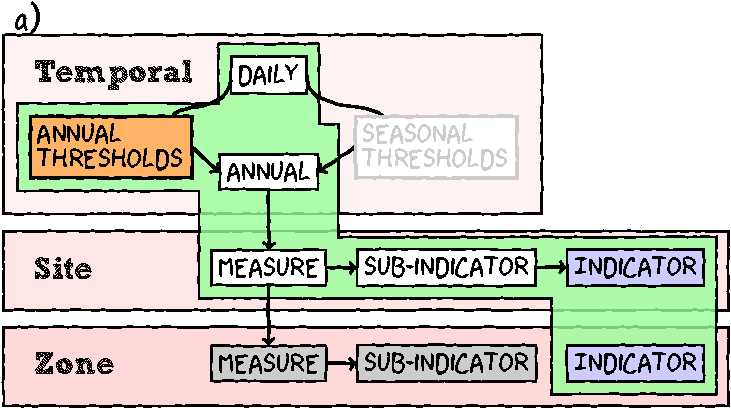
\includegraphics[width=0.49\linewidth]{figures/Diagrams/hier.pdf}
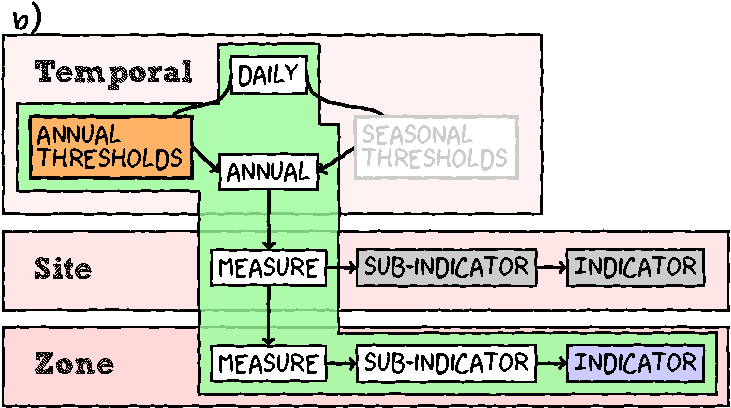
\includegraphics[width=0.49\linewidth]{figures/Diagrams/hier1.pdf}\\\\[1em]
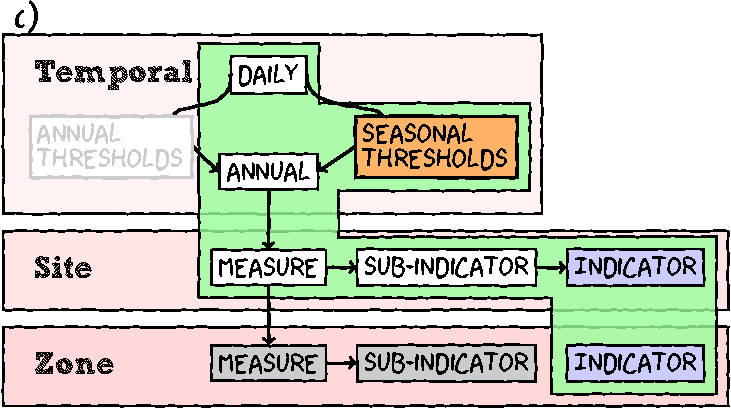
\includegraphics[width=0.49\linewidth]{figures/Diagrams/hier2.pdf}
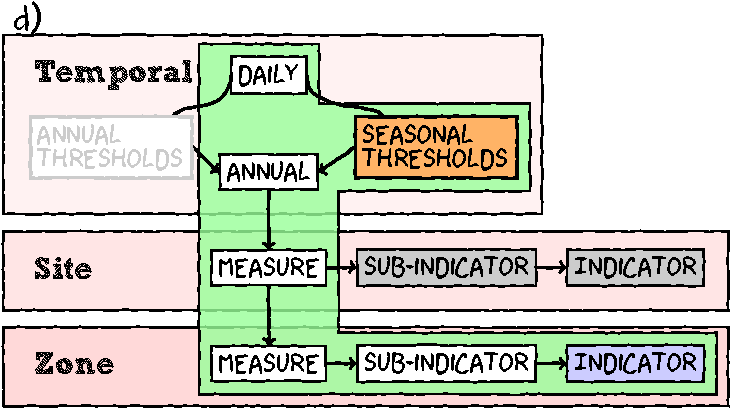
\includegraphics[width=0.49\linewidth]{figures/Diagrams/hier3.pdf}
\caption[Agregation sequence schematic]{Schematic illustrating four possible aggregation routines through the combination of Temporal (Daily, Seasonal and Annual), Spatial (Site, Zone) and Measure 
(Measure, Sub-indicator, Indicator) nodes of the triple hierarchical
aggregation routine associated with the GBR Report Card. Aggregation directions between 
nodes are signified by arrows and the main aggregation pathway through
the routines is illustrated by the green polygon. }\label{fig:hier}
\end{figure}
\end{landscape}
       



To maximize information retention throughout a series of aggregations, it is preferable to aggregate
distributions rather than single properties of those distributions (such as means). The simplest way
to perform a hierarchy of aggregations is to interactively calculate the means (or median) of items
(means of means etc). At each successive aggregation level only very basic distributional summaries
(such as the mean and perhaps standard deviation) are retained, the bulk of upstream information is
lost. Alternatively, more complex methods that involve combining data or probability distributions
can be effective at aggregating data in a way that propagates rich distributional properties
throughout a series of aggregations.

Importantly, if the purpose of aggregation is purely to establish a new point estimate of the
combined items, a large variety of methods essentially yield the same outcomes. On the other hand,
if the purpose of aggregation is also to propagate a measure of uncertainty or confidence in the
point estimate through multiple hierarchical levels of aggregation (as is the case here), then the
different methodologies offer differing degrees of flexibility and suitability.

Hierarchical aggregations are essentially a series of steps that sequentially combine distributions
(which progressively become more data rich). The resulting distribution formed at each step should
thereby reflect the general conditions typified by its parent distributions and by extension, each
of the distributions higher up the hierarchy.

Numerous characteristics can be estimated from a distribution including the location (such as mean
and median) and scale (such as variance and range). For the current project, the mean and variance
were considered the most appropriate\footnote{The aggregations typically involve some Measures with
a small number of unique observations (and thus indices) and thus means and variances provide
greater sensitivity than medians and ranges.  Moreover, the indexing stage effectively removes
outliers and standardizes the scale range thereby reducing the need for robust estimators.}
distributional descriptions and from these estimates Grades and measures of confidence can be
respectively derived. Hence the numerical summaries (mean and variance) at any stage of the
hierarchical aggregation are a byproduct rather than the sole property of propagation.


\subsubsection{Bootstrap aggregation}

Although some of the items to be aggregated together might initially comprise only a few values (or
even a single value), it is useful to conceptualize them as continuous distributions. For example,
when aggregating multiple \emph{Measures} (such as all Water Quality Chemicals) together to generate
a (\emph{Site} level) \emph{Sub-indicator} average, each \emph{Measure} in each \emph{Site} can be
considered a distribution comprising the single Score for that \emph{Measure}. Aggregation then
involves combining together the multiple distributions into a single amalgam (by adding the
distributions together, see Figure \ref{fig:bootstrap}). Similarly, when aggregating at the
\emph{Indicator} level across \emph{Site} to generate \emph{Zone} summaries for each
\emph{Indicator}, \emph{Site} distributions are respectively added together to yield a single
distribution per \emph{Zone}.

\begin{figure}[h]
\centering
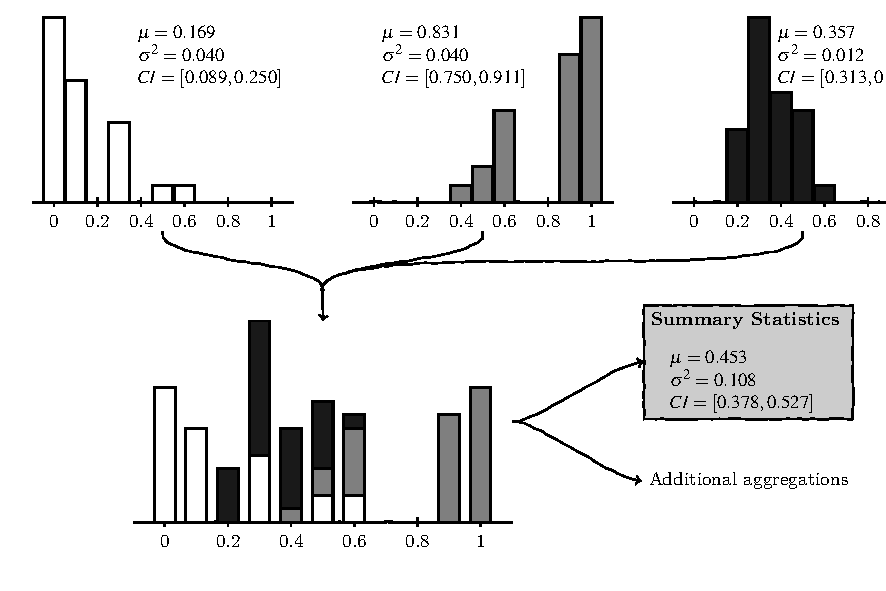
\includegraphics[width=0.7\linewidth]{figures/Diagrams/bootstrap.pdf}
\caption[Bootstrap aggregation schematic]{Illustration of Bootstrapped aggregation of three distributions.  Simple summary statistics (mean, variance and 95\% confidence interval presented for each distribution).}\label{fig:bootstrap}
\end{figure}


If the distributions being aggregated are all proportional distributions (e.g.~density
distributions), adding them altogether is trivially simple. However, if, rather than actual
distributions, the items to be aggregated are actually just small collections of values (as is the
case for many of the discrete Measures here) or even large, yet unequally populous collections of
values (as could be the case for Continuous Flow Monitoring with missing or suspect observations),
then simply aggregating the distributions together will result in amalgams that are weighted
according to the size of the collections (larger collections will have more influence). For example,
if we were aggregating together three \emph{Zones} (to yield Whole GBR estimates), one of which
comprised twice as many Sites, simple aggregation of distributions would result in a distribution
that was more highly influenced by the Zone with the more \emph{Sites}. Similarly, when aggregating
from the level of Sub-indicator to the level of Indicator, the resulting Indicator would be biased
towards the Sub-indicator with the most Measures.  Whilst this may well be a useful property
(e.g.~stratified aggregation), it may also be undesirable.

Bootstrapping is a simulation process that involves repeated sampling (in this case with
replacement) of a sample set with the aim of generating a bootstrap sample from a distribution.
This bootstrap sample can be used to estimate the underlying probability distribution function that
generated the data as well as any other summary statistics.  Importantly, bootstrapping provides a
way to generate distributions that are proportional and thus un-weighted by the original sample
sizes thereby facilitating un-weighted aggregation\footnote{technically, all equally weighted rather
than un-weighted}.  Bootstrapped distributions can be aggregated (added together) to yield
accumulated child distributions that retain the combined properties of both parents (see Figure
\ref{fig:bootstrap}). As a stochastic process, repeated calculations will yield slightly different
outcomes. Nevertheless, the more bootstrap samples are collected, the greater the bootstrap
distributions will reflect the underlying Score distribution and provided the number of drawn
samples is sufficiently large (e.g. 10,000 re-samples), repeated outcomes will converge.

To reiterate, the advantage of bootstrapping data before concatenating (or averaging) versus simply
concatenating data from multiple sources together, is to ensure that source data are all of exactly
the same sample size (so as to not weight more heavily towards the more populous
source(s)\footnote{Such weightings should be handled in other ways if at all}).  Bootstrapping also
provides a mechanism for propagating all distribution information throughout an aggregation
hierarchy and ensures that estimates of variance derived from child distributions are on a
consistent scale\footnote{Variance is inversely proportional to sample size}. The latter point is
absolutely critical if variance is going to be used to inform a Confidence Rating system and
confidence intervals.

Minimum operator procedures are supported by filtering on the lowest performed indicator prior to
bootstrapping. Importantly, the bootstrapping routine simply provides a mechanism to collate all
sources together to yield a super distribution. Thereafter, the joint distribution can be summarized
in what ever manner is deemed appropriate (arithmetic, geometric, harmonic means, medians, variance,
range, quantiles etc). Moreover, different levels of the aggregation can be summarized with
different statistics if appropriate.

\subsubsection{Beta approximation}

Whilst the bootstrap aggregation approach described above does offer a robust way to combine data
across scales and sources, for large data sets, it does impose large computational and storage
burdens.  For such cases (large data such as remote sensing), index distributions can be
approximated by beta distributions.  The beta distribution is defined on the interval [0,1] and is
parameterized by two positive shape parameters ($\alpha$, $\beta$) according to the following:
$$
f(x;\alpha, \beta) = \frac{\Gamma(\alpha +
\beta)}{\Gamma(\alpha)\Gamma(\beta)}x^{\alpha-1}(1-x)^{\beta-1}
$$

A beta function can manifest as many different shapes and as all of these are described by just two
shape parameters.  Therefore, rather than store all the bootstrapped values for each distribution,
we can alternatively approximate each distribution by a beta and store only the defining shape
parameters of each distribution.  When combining, rather than randomly sample 10,000 stored values
of each distribution, we simple resample 10,000 random draws from each beta
distribution\footnote{Unfortunately there is no closed-form general formula for the sum of multiple
independent beta distributions.}.  The combined distribution can then be approximated by a beta
distribution and so on.

\begin{figure}[ht]
\begin{center}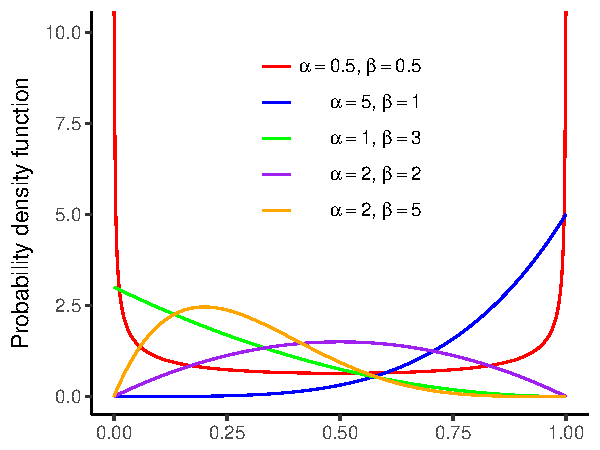
\includegraphics{figures/Diagrams/beta.pdf}\end{center}
\caption{Beta probability densities}\label{fig:beta}
\end{figure}

\subsubsection{Weights}



Standard bootstrapping yields equally weighted distributions, however, specific weighting schemes
can also be easily applied by bootstrapping in proportion to the weights. For example, to weight one
parent twice as high as another, simply collect twice as many re-samples from the first
distribution. To ensure that all resulting distributions have the same size (by default 10,000
items), the number of bootstrap samples collected ($n$) from each of the ($p$) parent distributions
($i$), given the weights ($w_i$) is calculated as:
$$
n_i=\ceil{(S/p)\times w_i}
$$ 
where $S$ is the target size (10,000) and $\ceil{.}$ indicates the ceiling.  Qualitative data (such
as ratings) can also be incorporated by enumerating the categories before bootstrapping.


In addition to allowing expert driven weights that govern the contribution of different items during
aggregations, it is possible to weight according to relative spatial areas during spatial
aggregations.  Currently, all Sites are equally weighted when aggregating to Zone level and all
Zones equal when aggregating to Whole of GBR level.  That means that small Zones have an equal
contribution as large Zones despite representing a smaller fraction of the water body.  Area based
weights could be applied such that Sites and Zones contribute in proportion to relative areas.

Weights are defined by a user editable configuration file that is similar in structure to the Water
Quality thresholds file.


\subsubsection{Expert interventions}

The ability for experts and Report Card managers to intervene (exclude or overwrite) Scores/Grades
at any Spatial/Measure scale is essential to maintain the quality of a Report Card in the event of
unrepresentative or suspect data.  The current system is able to support expert interventions in the
form of exclusions and overwrites.  For example, after reviewing the QAQC, an expert can elect to
exclude one or more Measures (or Subindicators etc) from one or more spatial scales.  Such
interventions are specified via a user editable configuration files\footnote{Since aggregation
occurs across two hierarchies (the Measure hierarchy and the Spatial hierarchy - see Figures
\ref{fig:hierarchies} and \ref{fig:hier}), two configuration files are necessary.} (csv) that is
similar in structure to the Water Quality thresholds file.

The essential component of this configuration file is that it allows a user to specify what Data are
to be excluded or replaced. These can be at any of the levels of the Measure hierarchy (Measures,
Sub-indications and Indicators) and any level of the Spatial hierarchy (Sites, Zones and Whole GBR).
Settings pertaining to levels further along the aggregation hierarchies have precedence. For
example, if Chemicals are excluded (or overridden) in a particular Zone, then all Chemical Measures
within all Sites will be excluded irrespective of what the settings are for any specific
Measure/Site.

\subsubsection{Scores and Grades}

The double hierarchy Bootstrap aggregation described above, yields \textbf{Score} distributions for
each Measure-level/Spatial-level combination. The location and scale of each distribution can thus
be described by its mean and variance. Mean \textbf{Scores} are then converted into a simple
five-point alphanumeric \textbf{Grade} scale (and associated colors) using a control chart (see
Figure~\ref{fig:control}).

\begin{figure}[ht]
  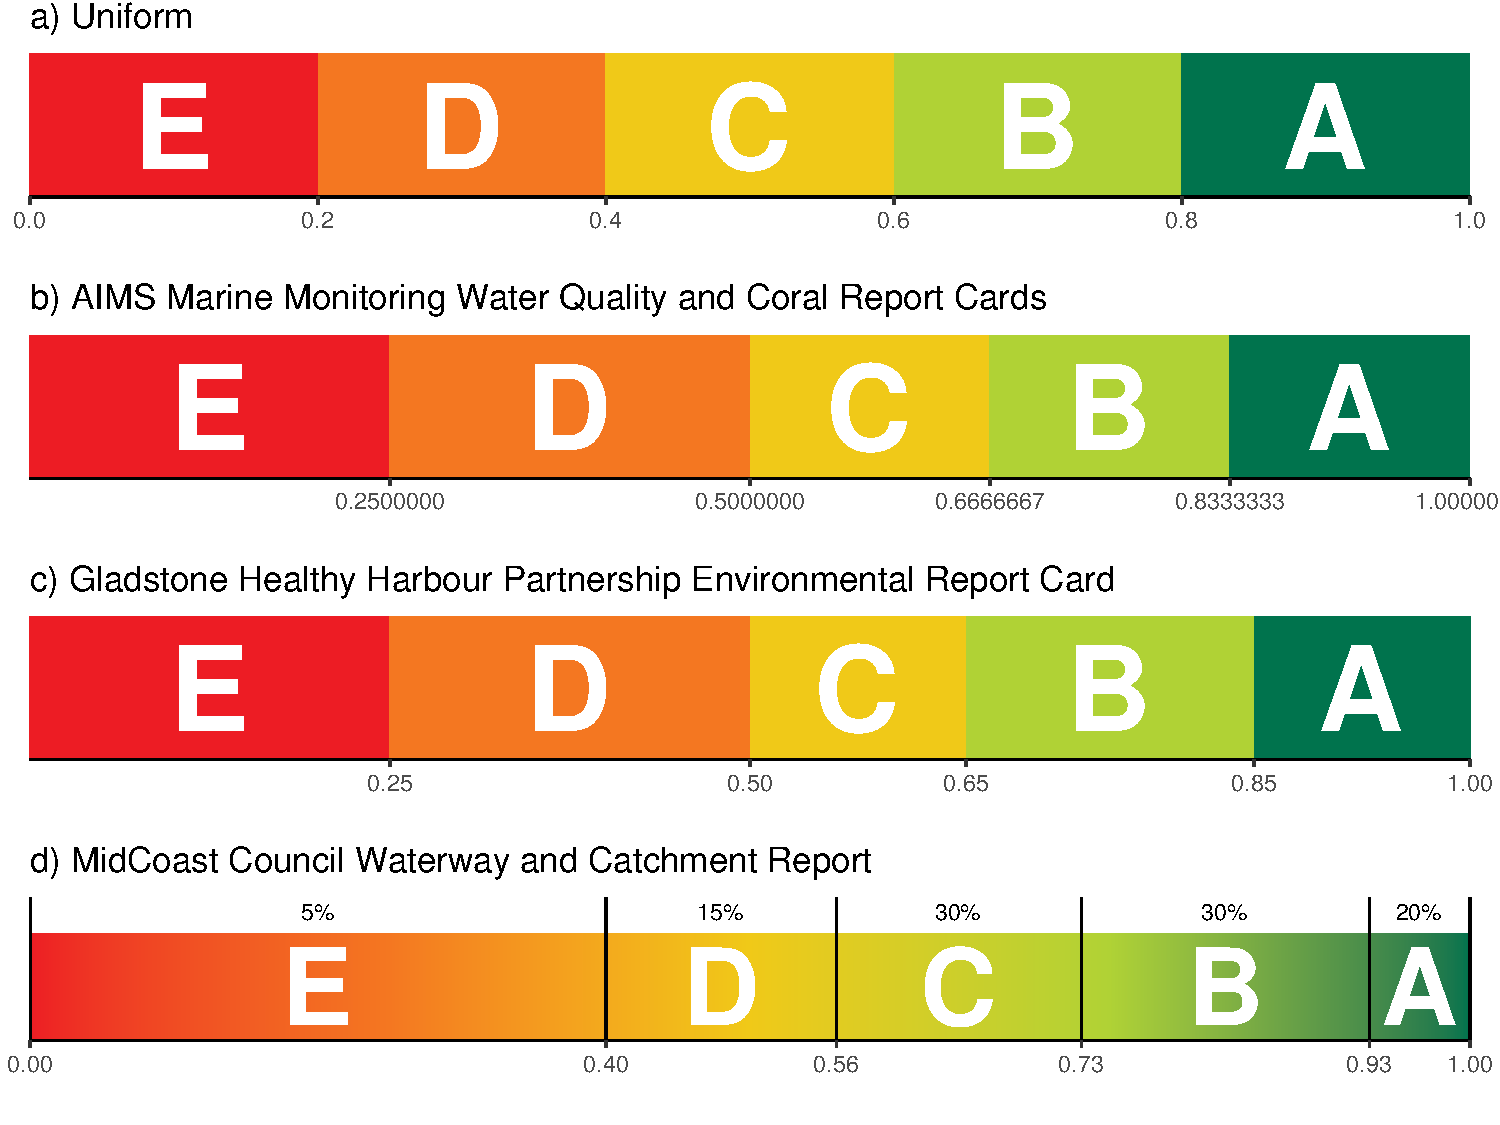
\includegraphics[width=\linewidth]{figures/Diagrams/controlcharts.pdf}
  \caption{Score to grade conversion control charts.  In each case, the scale along the base defines the grade
  boundaries.}\label{fig:control}
\end{figure}

The control charts adopted by the AIMS inshore water quality Marine Monitoring Program
\citep[MMP][]{Lonborg-MMP-2015} and the Gladstone Healthy Harbour Partnership \citep{GHHP-2016} both
define two levels (Poor and Very Poor) under the Threshold values and three above (Satisfactory,
Good and Very Good).  The threshold is purposely placed at the boundary of two grades so as to ease
the distinction between 'pass' and 'fail'.  The major difference between these two charts is that
whereas the AIMS MMP report card control chart partitions the three better than threshold
categories, the Gladstone Healthy Harbour Partnership report card control chart employs simpler
boundary cutoffs around the 'B' grade (although this does result in arbitrarily unequal category
sizes.

By contrast, the MidCoast Council (formally Great Lakes Council) Waterway and Catchment Report
\citep{MidCoastCouncil-2016} uses grade boundaries based on historical score distribution quantiles
associated with definitions of what proportion of total observations (sites) are considered
'Excellent' (A), 'Good' (B), 'Fair' (C), 'Poor' (D) and 'Very Poor' (Fig.~\ref{fig:control}d).  For
example, the 'Very Poor' grade was defined as the worst 5\% of sites across the entire State of New
South Wales and the lowest 5\% of sites has a maximum score of 0.4.  This approach recognizes the
non-linear spread of scores resulting from their particular metrics and attempts to ensure that
grades are intuitively interpretable (A grade of A means the site is in Excellent condition).
Nevertheless, it does necessitate a of historical data and as well as a very specific and agreed
upon set of a priori condition definitions.

% \begin{table}[ht]
% \centering\scriptsize\scriptsize
% \caption{GBR Report Card Grade scale control chart.} 
% \label{tab:control}
% \begin{tabular}{rcl}
%   \toprule
% {\textbf{Score}} & {\textbf{Grade}} & {\textbf{Description}} \\ 
%   \midrule
% $\ge 0.80$ & \cellcolor[HTML]{00734D}{A} & Very Good \\ 
%   $\ge 0.60, <0.80$ & \cellcolor[HTML]{B0D235}{B} & Good \\ 
%   $\ge 0.40, <0.60$ & \cellcolor[HTML]{F0C918}{C} & Satisfactory \\ 
%   $\geq 0.20, < 0.40$ & \cellcolor[HTML]{F47721}{D} & Poor \\ 
%   $<0.20$ & \cellcolor[HTML]{ED1C24}{E} & Very Poor \\ 
%    \bottomrule
% \end{tabular}
% \end{table}

In each of the above approaches, grade boundaries are usually determined to some extent by expert
panel to ensure that the range of indices represented by each grade classification is congruent with
community interpretation of a letter grade report cards. It is far less clear how estimates of
uncertainty can be incorporated into such a grading scheme in a manner that will be intuitive to
non-technical audiences. That said, statistical uncertainty is just one of many sources of un-
certainty that should be captured into a confidence or certainty rating. Hence any expectations of
presenting uncertainty in a quantitative manner may well be unrealistic anyway.

In the absence of expert opinion, we have elected to adopt a very simple score-grade control chart
in which the score range is simply partitioned into five equal grades (Fig.~\ref{fig:control}a).


\subsubsection{Certainty rating}

Incorporating an estimate of scale (variance) into a certainty or confidence rating necessitates
re-scaling the estimates into a standard scale. In particular, whereas a scale parameter of high
magnitude indicates lower degrees of certainty, for a certainty rating to be useful for end users,
larger numbers should probably represent higher degrees of certainty. Thus, the scaling process
should also reverse the scale. Furthermore, variance is dependent on the magnitude of the values.

In order to re-scale a scale estimate into a certainty rating, it is necessary to establish the
range of values possible for the scale estimate. Whilst the minimum is simple enough (it will
typically be 0), determining the maximum is a little more challenging depending on the aggregation
algorithm (bootstrapping, Bayesian Network etc). One of the advantages in utilizing proportional
distributions (such as is the case for a Bayesian Network or a re-sampled bootstrap distribution) is
that the scale parameter for the single worst case scenario can be devised (once the worst case
scenario has been determined) independent of sample sizes or weightings. In most situations this is
going to be when the distribution comprises equal mass at (and only at) each of the two extremes
(for example, values of just 0 and 1).

The measure of confidence rating discussed above is purely an objective metric derived from the
variance in the aggregation hierarchy. It is completely naive to issues such as missing data,
outliers and Limit of Detection issues - the influences of which on a confidence rating are
necessarily subjective. A full Confidence Rating would combine these objective variance component
with additional subjective considerations such as climatic and disturbance information, and the
perceived influence of missing, Limit of Detection and outlying data. Hence, the statistical scaled
statistical variance would form just one component in the Confidence Rating system.

The bootstrap aggregation method provides a mechanism for estimating variance from which to build
such an expert considered Confidence Rating system.
  

Table~\ref{tab:GradeTypeComparisons} presents the Water Quality Indicator Scores and associated
Grades for each Zone based on three of the grade control chart types described in
Figure~\ref{fig:control} for the eReefs data indexed using the fsMAMP formulation.  Whilst there is
some agreement between the different grade types, in general, the Uniform type yields higher grades
than either MMP or GHHP.

  
\sf
\LTcapwidth=\linewidth
\setlength\aboverulesep{0pt}\setlength\belowrulesep{0pt}
\setlength\cmidrulekern{1pt}\setlength\cmidrulewidth{1pt}
\renewcommand\arraystretch{1.2}\setlength\tabcolsep{5pt}
{
\small
\begin{longtable}{llccccc}
\caption{Score and associated Grades based on three different grade control charts (Uniform, MMP and GHHP) for eReefs data indexed via fsMAMP and aggregated to Zone/Indicator level.}\label{tab:GradeTypeComparisons}\\ 
\toprule
Region&Water Body & Water Year & Score & Grade (MMP) & Grade (Uniform) & Grade (GHHP)\\
\midrule
\endfirsthead
\multicolumn{7}{l}{..continued from previous page}\\
\toprule
Region&Water Body & Water Year & Score & Grade (MMP) & Grade (Uniform) & Grade (GHHP)\\
\midrule 

\endhead Cape York & Open Coastal & 2014 & 0.692 & \cellcolor[HTML]{B0D235}{B} & \cellcolor[HTML]{B0D235}{B} & \cellcolor[HTML]{B0D235}{B} \\ 
  Cape York & Open Coastal & 2014 & 0.791 & \cellcolor[HTML]{B0D235}{B} & \cellcolor[HTML]{B0D235}{B} & \cellcolor[HTML]{B0D235}{B} \\ 
  Cape York & Open Coastal & 2014 & 0.891 & \cellcolor[HTML]{00734D}{A} & \cellcolor[HTML]{00734D}{A} & \cellcolor[HTML]{00734D}{A} \\ 
  Cape York & Open Coastal & 2014 & 0.856 & \cellcolor[HTML]{00734D}{A} & \cellcolor[HTML]{00734D}{A} & \cellcolor[HTML]{00734D}{A} \\ 
  Cape York & Open Coastal & 2015 & 0.741 & \cellcolor[HTML]{B0D235}{B} & \cellcolor[HTML]{B0D235}{B} & \cellcolor[HTML]{B0D235}{B} \\ 
  Cape York & Open Coastal & 2015 & 0.824 & \cellcolor[HTML]{B0D235}{B} & \cellcolor[HTML]{00734D}{A} & \cellcolor[HTML]{B0D235}{B} \\ 
  Cape York & Open Coastal & 2015 & 0.906 & \cellcolor[HTML]{00734D}{A} & \cellcolor[HTML]{00734D}{A} & \cellcolor[HTML]{00734D}{A} \\ 
  Cape York & Open Coastal & 2015 & 0.880 & \cellcolor[HTML]{00734D}{A} & \cellcolor[HTML]{00734D}{A} & \cellcolor[HTML]{00734D}{A} \\ 
  Cape York & Open Coastal & 2016 & 0.757 & \cellcolor[HTML]{B0D235}{B} & \cellcolor[HTML]{B0D235}{B} & \cellcolor[HTML]{B0D235}{B} \\ 
  Cape York & Open Coastal & 2016 & 0.837 & \cellcolor[HTML]{00734D}{A} & \cellcolor[HTML]{00734D}{A} & \cellcolor[HTML]{B0D235}{B} \\ 
  Cape York & Open Coastal & 2016 & 0.917 & \cellcolor[HTML]{00734D}{A} & \cellcolor[HTML]{00734D}{A} & \cellcolor[HTML]{00734D}{A} \\ 
  Cape York & Open Coastal & 2016 & 0.891 & \cellcolor[HTML]{00734D}{A} & \cellcolor[HTML]{00734D}{A} & \cellcolor[HTML]{00734D}{A} \\ 
  Cape York & Midshelf & 2014 & 0.716 & \cellcolor[HTML]{B0D235}{B} & \cellcolor[HTML]{B0D235}{B} & \cellcolor[HTML]{B0D235}{B} \\ 
  Cape York & Midshelf & 2014 & 0.805 & \cellcolor[HTML]{B0D235}{B} & \cellcolor[HTML]{00734D}{A} & \cellcolor[HTML]{B0D235}{B} \\ 
  Cape York & Midshelf & 2014 & 0.894 & \cellcolor[HTML]{00734D}{A} & \cellcolor[HTML]{00734D}{A} & \cellcolor[HTML]{00734D}{A} \\ 
  Cape York & Midshelf & 2014 & 0.862 & \cellcolor[HTML]{00734D}{A} & \cellcolor[HTML]{00734D}{A} & \cellcolor[HTML]{00734D}{A} \\ 
  Cape York & Midshelf & 2015 & 0.764 & \cellcolor[HTML]{B0D235}{B} & \cellcolor[HTML]{B0D235}{B} & \cellcolor[HTML]{B0D235}{B} \\ 
  Cape York & Midshelf & 2015 & 0.838 & \cellcolor[HTML]{00734D}{A} & \cellcolor[HTML]{00734D}{A} & \cellcolor[HTML]{B0D235}{B} \\ 
  Cape York & Midshelf & 2015 & 0.913 & \cellcolor[HTML]{00734D}{A} & \cellcolor[HTML]{00734D}{A} & \cellcolor[HTML]{00734D}{A} \\ 
  Cape York & Midshelf & 2015 & 0.891 & \cellcolor[HTML]{00734D}{A} & \cellcolor[HTML]{00734D}{A} & \cellcolor[HTML]{00734D}{A} \\ 
  Cape York & Midshelf & 2016 & 0.781 & \cellcolor[HTML]{B0D235}{B} & \cellcolor[HTML]{B0D235}{B} & \cellcolor[HTML]{B0D235}{B} \\ 
  Cape York & Midshelf & 2016 & 0.855 & \cellcolor[HTML]{00734D}{A} & \cellcolor[HTML]{00734D}{A} & \cellcolor[HTML]{00734D}{A} \\ 
  Cape York & Midshelf & 2016 & 0.929 & \cellcolor[HTML]{00734D}{A} & \cellcolor[HTML]{00734D}{A} & \cellcolor[HTML]{00734D}{A} \\ 
  Cape York & Midshelf & 2016 & 0.903 & \cellcolor[HTML]{00734D}{A} & \cellcolor[HTML]{00734D}{A} & \cellcolor[HTML]{00734D}{A} \\ 
  Cape York & Offshore & 2014 & 0.825 & \cellcolor[HTML]{B0D235}{B} & \cellcolor[HTML]{00734D}{A} & \cellcolor[HTML]{B0D235}{B} \\ 
  Cape York & Offshore & 2014 & 0.874 & \cellcolor[HTML]{00734D}{A} & \cellcolor[HTML]{00734D}{A} & \cellcolor[HTML]{00734D}{A} \\ 
  Cape York & Offshore & 2014 & 0.923 & \cellcolor[HTML]{00734D}{A} & \cellcolor[HTML]{00734D}{A} & \cellcolor[HTML]{00734D}{A} \\ 
  Cape York & Offshore & 2014 & 0.911 & \cellcolor[HTML]{00734D}{A} & \cellcolor[HTML]{00734D}{A} & \cellcolor[HTML]{00734D}{A} \\ 
  Cape York & Offshore & 2015 & 0.852 & \cellcolor[HTML]{00734D}{A} & \cellcolor[HTML]{00734D}{A} & \cellcolor[HTML]{00734D}{A} \\ 
  Cape York & Offshore & 2015 & 0.896 & \cellcolor[HTML]{00734D}{A} & \cellcolor[HTML]{00734D}{A} & \cellcolor[HTML]{00734D}{A} \\ 
  Cape York & Offshore & 2015 & 0.941 & \cellcolor[HTML]{00734D}{A} & \cellcolor[HTML]{00734D}{A} & \cellcolor[HTML]{00734D}{A} \\ 
  Cape York & Offshore & 2015 & 0.928 & \cellcolor[HTML]{00734D}{A} & \cellcolor[HTML]{00734D}{A} & \cellcolor[HTML]{00734D}{A} \\ 
  Cape York & Offshore & 2016 & 0.895 & \cellcolor[HTML]{00734D}{A} & \cellcolor[HTML]{00734D}{A} & \cellcolor[HTML]{00734D}{A} \\ 
  Cape York & Offshore & 2016 & 0.927 & \cellcolor[HTML]{00734D}{A} & \cellcolor[HTML]{00734D}{A} & \cellcolor[HTML]{00734D}{A} \\ 
  Cape York & Offshore & 2016 & 0.960 & \cellcolor[HTML]{00734D}{A} & \cellcolor[HTML]{00734D}{A} & \cellcolor[HTML]{00734D}{A} \\ 
  Cape York & Offshore & 2016 & 0.951 & \cellcolor[HTML]{00734D}{A} & \cellcolor[HTML]{00734D}{A} & \cellcolor[HTML]{00734D}{A} \\ 
  Wet Tropics & Open Coastal & 2014 & 0.602 & \cellcolor[HTML]{F0C918}{C} & \cellcolor[HTML]{B0D235}{B} & \cellcolor[HTML]{F0C918}{C} \\ 
  Wet Tropics & Open Coastal & 2014 & 0.711 & \cellcolor[HTML]{B0D235}{B} & \cellcolor[HTML]{B0D235}{B} & \cellcolor[HTML]{B0D235}{B} \\ 
  Wet Tropics & Open Coastal & 2014 & 0.819 & \cellcolor[HTML]{B0D235}{B} & \cellcolor[HTML]{00734D}{A} & \cellcolor[HTML]{B0D235}{B} \\ 
  Wet Tropics & Open Coastal & 2014 & 0.742 & \cellcolor[HTML]{B0D235}{B} & \cellcolor[HTML]{B0D235}{B} & \cellcolor[HTML]{B0D235}{B} \\ 
  Wet Tropics & Open Coastal & 2015 & 0.668 & \cellcolor[HTML]{B0D235}{B} & \cellcolor[HTML]{B0D235}{B} & \cellcolor[HTML]{B0D235}{B} \\ 
  Wet Tropics & Open Coastal & 2015 & 0.760 & \cellcolor[HTML]{B0D235}{B} & \cellcolor[HTML]{B0D235}{B} & \cellcolor[HTML]{B0D235}{B} \\ 
  Wet Tropics & Open Coastal & 2015 & 0.853 & \cellcolor[HTML]{00734D}{A} & \cellcolor[HTML]{00734D}{A} & \cellcolor[HTML]{00734D}{A} \\ 
  Wet Tropics & Open Coastal & 2015 & 0.803 & \cellcolor[HTML]{B0D235}{B} & \cellcolor[HTML]{00734D}{A} & \cellcolor[HTML]{B0D235}{B} \\ 
  Wet Tropics & Open Coastal & 2016 & 0.692 & \cellcolor[HTML]{B0D235}{B} & \cellcolor[HTML]{B0D235}{B} & \cellcolor[HTML]{B0D235}{B} \\ 
  Wet Tropics & Open Coastal & 2016 & 0.790 & \cellcolor[HTML]{B0D235}{B} & \cellcolor[HTML]{B0D235}{B} & \cellcolor[HTML]{B0D235}{B} \\ 
  Wet Tropics & Open Coastal & 2016 & 0.888 & \cellcolor[HTML]{00734D}{A} & \cellcolor[HTML]{00734D}{A} & \cellcolor[HTML]{00734D}{A} \\ 
  Wet Tropics & Open Coastal & 2016 & 0.836 & \cellcolor[HTML]{00734D}{A} & \cellcolor[HTML]{00734D}{A} & \cellcolor[HTML]{B0D235}{B} \\ 
  Wet Tropics & Midshelf & 2014 & 0.711 & \cellcolor[HTML]{B0D235}{B} & \cellcolor[HTML]{B0D235}{B} & \cellcolor[HTML]{B0D235}{B} \\ 
  Wet Tropics & Midshelf & 2014 & 0.789 & \cellcolor[HTML]{B0D235}{B} & \cellcolor[HTML]{B0D235}{B} & \cellcolor[HTML]{B0D235}{B} \\ 
  Wet Tropics & Midshelf & 2014 & 0.866 & \cellcolor[HTML]{00734D}{A} & \cellcolor[HTML]{00734D}{A} & \cellcolor[HTML]{00734D}{A} \\ 
  Wet Tropics & Midshelf & 2014 & 0.826 & \cellcolor[HTML]{B0D235}{B} & \cellcolor[HTML]{00734D}{A} & \cellcolor[HTML]{B0D235}{B} \\ 
  Wet Tropics & Midshelf & 2015 & 0.760 & \cellcolor[HTML]{B0D235}{B} & \cellcolor[HTML]{B0D235}{B} & \cellcolor[HTML]{B0D235}{B} \\ 
  Wet Tropics & Midshelf & 2015 & 0.826 & \cellcolor[HTML]{B0D235}{B} & \cellcolor[HTML]{00734D}{A} & \cellcolor[HTML]{B0D235}{B} \\ 
  Wet Tropics & Midshelf & 2015 & 0.893 & \cellcolor[HTML]{00734D}{A} & \cellcolor[HTML]{00734D}{A} & \cellcolor[HTML]{00734D}{A} \\ 
  Wet Tropics & Midshelf & 2015 & 0.866 & \cellcolor[HTML]{00734D}{A} & \cellcolor[HTML]{00734D}{A} & \cellcolor[HTML]{00734D}{A} \\ 
  Wet Tropics & Midshelf & 2016 & 0.796 & \cellcolor[HTML]{B0D235}{B} & \cellcolor[HTML]{B0D235}{B} & \cellcolor[HTML]{B0D235}{B} \\ 
  Wet Tropics & Midshelf & 2016 & 0.864 & \cellcolor[HTML]{00734D}{A} & \cellcolor[HTML]{00734D}{A} & \cellcolor[HTML]{00734D}{A} \\ 
  Wet Tropics & Midshelf & 2016 & 0.933 & \cellcolor[HTML]{00734D}{A} & \cellcolor[HTML]{00734D}{A} & \cellcolor[HTML]{00734D}{A} \\ 
  Wet Tropics & Midshelf & 2016 & 0.905 & \cellcolor[HTML]{00734D}{A} & \cellcolor[HTML]{00734D}{A} & \cellcolor[HTML]{00734D}{A} \\ 
  Wet Tropics & Offshore & 2014 & 0.819 & \cellcolor[HTML]{B0D235}{B} & \cellcolor[HTML]{00734D}{A} & \cellcolor[HTML]{B0D235}{B} \\ 
  Wet Tropics & Offshore & 2014 & 0.868 & \cellcolor[HTML]{00734D}{A} & \cellcolor[HTML]{00734D}{A} & \cellcolor[HTML]{00734D}{A} \\ 
  Wet Tropics & Offshore & 2014 & 0.918 & \cellcolor[HTML]{00734D}{A} & \cellcolor[HTML]{00734D}{A} & \cellcolor[HTML]{00734D}{A} \\ 
  Wet Tropics & Offshore & 2014 & 0.906 & \cellcolor[HTML]{00734D}{A} & \cellcolor[HTML]{00734D}{A} & \cellcolor[HTML]{00734D}{A} \\ 
  Wet Tropics & Offshore & 2015 & 0.844 & \cellcolor[HTML]{00734D}{A} & \cellcolor[HTML]{00734D}{A} & \cellcolor[HTML]{B0D235}{B} \\ 
  Wet Tropics & Offshore & 2015 & 0.886 & \cellcolor[HTML]{00734D}{A} & \cellcolor[HTML]{00734D}{A} & \cellcolor[HTML]{00734D}{A} \\ 
  Wet Tropics & Offshore & 2015 & 0.929 & \cellcolor[HTML]{00734D}{A} & \cellcolor[HTML]{00734D}{A} & \cellcolor[HTML]{00734D}{A} \\ 
  Wet Tropics & Offshore & 2015 & 0.923 & \cellcolor[HTML]{00734D}{A} & \cellcolor[HTML]{00734D}{A} & \cellcolor[HTML]{00734D}{A} \\ 
  Wet Tropics & Offshore & 2016 & 0.873 & \cellcolor[HTML]{00734D}{A} & \cellcolor[HTML]{00734D}{A} & \cellcolor[HTML]{00734D}{A} \\ 
  Wet Tropics & Offshore & 2016 & 0.910 & \cellcolor[HTML]{00734D}{A} & \cellcolor[HTML]{00734D}{A} & \cellcolor[HTML]{00734D}{A} \\ 
  Wet Tropics & Offshore & 2016 & 0.947 & \cellcolor[HTML]{00734D}{A} & \cellcolor[HTML]{00734D}{A} & \cellcolor[HTML]{00734D}{A} \\ 
  Wet Tropics & Offshore & 2016 & 0.940 & \cellcolor[HTML]{00734D}{A} & \cellcolor[HTML]{00734D}{A} & \cellcolor[HTML]{00734D}{A} \\ 
  Dry Tropics & Open Coastal & 2014 & 0.580 & \cellcolor[HTML]{F0C918}{C} & \cellcolor[HTML]{F0C918}{C} & \cellcolor[HTML]{F0C918}{C} \\ 
  Dry Tropics & Open Coastal & 2014 & 0.686 & \cellcolor[HTML]{B0D235}{B} & \cellcolor[HTML]{B0D235}{B} & \cellcolor[HTML]{B0D235}{B} \\ 
  Dry Tropics & Open Coastal & 2014 & 0.793 & \cellcolor[HTML]{B0D235}{B} & \cellcolor[HTML]{B0D235}{B} & \cellcolor[HTML]{B0D235}{B} \\ 
  Dry Tropics & Open Coastal & 2014 & 0.772 & \cellcolor[HTML]{B0D235}{B} & \cellcolor[HTML]{B0D235}{B} & \cellcolor[HTML]{B0D235}{B} \\ 
  Dry Tropics & Open Coastal & 2015 & 0.624 & \cellcolor[HTML]{F0C918}{C} & \cellcolor[HTML]{B0D235}{B} & \cellcolor[HTML]{F0C918}{C} \\ 
  Dry Tropics & Open Coastal & 2015 & 0.726 & \cellcolor[HTML]{B0D235}{B} & \cellcolor[HTML]{B0D235}{B} & \cellcolor[HTML]{B0D235}{B} \\ 
  Dry Tropics & Open Coastal & 2015 & 0.829 & \cellcolor[HTML]{B0D235}{B} & \cellcolor[HTML]{00734D}{A} & \cellcolor[HTML]{B0D235}{B} \\ 
  Dry Tropics & Open Coastal & 2015 & 0.813 & \cellcolor[HTML]{B0D235}{B} & \cellcolor[HTML]{00734D}{A} & \cellcolor[HTML]{B0D235}{B} \\ 
  Dry Tropics & Open Coastal & 2016 & 0.639 & \cellcolor[HTML]{F0C918}{C} & \cellcolor[HTML]{B0D235}{B} & \cellcolor[HTML]{F0C918}{C} \\ 
  Dry Tropics & Open Coastal & 2016 & 0.746 & \cellcolor[HTML]{B0D235}{B} & \cellcolor[HTML]{B0D235}{B} & \cellcolor[HTML]{B0D235}{B} \\ 
  Dry Tropics & Open Coastal & 2016 & 0.852 & \cellcolor[HTML]{00734D}{A} & \cellcolor[HTML]{00734D}{A} & \cellcolor[HTML]{00734D}{A} \\ 
  Dry Tropics & Open Coastal & 2016 & 0.827 & \cellcolor[HTML]{B0D235}{B} & \cellcolor[HTML]{00734D}{A} & \cellcolor[HTML]{B0D235}{B} \\ 
  Dry Tropics & Midshelf & 2014 & 0.758 & \cellcolor[HTML]{B0D235}{B} & \cellcolor[HTML]{B0D235}{B} & \cellcolor[HTML]{B0D235}{B} \\ 
  Dry Tropics & Midshelf & 2014 & 0.806 & \cellcolor[HTML]{B0D235}{B} & \cellcolor[HTML]{00734D}{A} & \cellcolor[HTML]{B0D235}{B} \\ 
  Dry Tropics & Midshelf & 2014 & 0.853 & \cellcolor[HTML]{00734D}{A} & \cellcolor[HTML]{00734D}{A} & \cellcolor[HTML]{00734D}{A} \\ 
  Dry Tropics & Midshelf & 2014 & 0.817 & \cellcolor[HTML]{B0D235}{B} & \cellcolor[HTML]{00734D}{A} & \cellcolor[HTML]{B0D235}{B} \\ 
  Dry Tropics & Midshelf & 2015 & 0.799 & \cellcolor[HTML]{B0D235}{B} & \cellcolor[HTML]{B0D235}{B} & \cellcolor[HTML]{B0D235}{B} \\ 
  Dry Tropics & Midshelf & 2015 & 0.841 & \cellcolor[HTML]{00734D}{A} & \cellcolor[HTML]{00734D}{A} & \cellcolor[HTML]{B0D235}{B} \\ 
  Dry Tropics & Midshelf & 2015 & 0.884 & \cellcolor[HTML]{00734D}{A} & \cellcolor[HTML]{00734D}{A} & \cellcolor[HTML]{00734D}{A} \\ 
  Dry Tropics & Midshelf & 2015 & 0.870 & \cellcolor[HTML]{00734D}{A} & \cellcolor[HTML]{00734D}{A} & \cellcolor[HTML]{00734D}{A} \\ 
  Dry Tropics & Midshelf & 2016 & 0.821 & \cellcolor[HTML]{B0D235}{B} & \cellcolor[HTML]{00734D}{A} & \cellcolor[HTML]{B0D235}{B} \\ 
  Dry Tropics & Midshelf & 2016 & 0.863 & \cellcolor[HTML]{00734D}{A} & \cellcolor[HTML]{00734D}{A} & \cellcolor[HTML]{00734D}{A} \\ 
  Dry Tropics & Midshelf & 2016 & 0.906 & \cellcolor[HTML]{00734D}{A} & \cellcolor[HTML]{00734D}{A} & \cellcolor[HTML]{00734D}{A} \\ 
  Dry Tropics & Midshelf & 2016 & 0.896 & \cellcolor[HTML]{00734D}{A} & \cellcolor[HTML]{00734D}{A} & \cellcolor[HTML]{00734D}{A} \\ 
  Dry Tropics & Offshore & 2014 & 0.778 & \cellcolor[HTML]{B0D235}{B} & \cellcolor[HTML]{B0D235}{B} & \cellcolor[HTML]{B0D235}{B} \\ 
  Dry Tropics & Offshore & 2014 & 0.842 & \cellcolor[HTML]{00734D}{A} & \cellcolor[HTML]{00734D}{A} & \cellcolor[HTML]{B0D235}{B} \\ 
  Dry Tropics & Offshore & 2014 & 0.907 & \cellcolor[HTML]{00734D}{A} & \cellcolor[HTML]{00734D}{A} & \cellcolor[HTML]{00734D}{A} \\ 
  Dry Tropics & Offshore & 2014 & 0.885 & \cellcolor[HTML]{00734D}{A} & \cellcolor[HTML]{00734D}{A} & \cellcolor[HTML]{00734D}{A} \\ 
  Dry Tropics & Offshore & 2015 & 0.809 & \cellcolor[HTML]{B0D235}{B} & \cellcolor[HTML]{00734D}{A} & \cellcolor[HTML]{B0D235}{B} \\ 
  Dry Tropics & Offshore & 2015 & 0.867 & \cellcolor[HTML]{00734D}{A} & \cellcolor[HTML]{00734D}{A} & \cellcolor[HTML]{00734D}{A} \\ 
  Dry Tropics & Offshore & 2015 & 0.924 & \cellcolor[HTML]{00734D}{A} & \cellcolor[HTML]{00734D}{A} & \cellcolor[HTML]{00734D}{A} \\ 
  Dry Tropics & Offshore & 2015 & 0.905 & \cellcolor[HTML]{00734D}{A} & \cellcolor[HTML]{00734D}{A} & \cellcolor[HTML]{00734D}{A} \\ 
  Dry Tropics & Offshore & 2016 & 0.829 & \cellcolor[HTML]{B0D235}{B} & \cellcolor[HTML]{00734D}{A} & \cellcolor[HTML]{B0D235}{B} \\ 
  Dry Tropics & Offshore & 2016 & 0.885 & \cellcolor[HTML]{00734D}{A} & \cellcolor[HTML]{00734D}{A} & \cellcolor[HTML]{00734D}{A} \\ 
  Dry Tropics & Offshore & 2016 & 0.940 & \cellcolor[HTML]{00734D}{A} & \cellcolor[HTML]{00734D}{A} & \cellcolor[HTML]{00734D}{A} \\ 
  Dry Tropics & Offshore & 2016 & 0.921 & \cellcolor[HTML]{00734D}{A} & \cellcolor[HTML]{00734D}{A} & \cellcolor[HTML]{00734D}{A} \\ 
  Mackay Whitsunday & Open Coastal & 2014 & 0.464 & \cellcolor[HTML]{F47721}{D} & \cellcolor[HTML]{F0C918}{C} & \cellcolor[HTML]{F47721}{D} \\ 
  Mackay Whitsunday & Open Coastal & 2014 & 0.559 & \cellcolor[HTML]{F0C918}{C} & \cellcolor[HTML]{F0C918}{C} & \cellcolor[HTML]{F0C918}{C} \\ 
  Mackay Whitsunday & Open Coastal & 2014 & 0.654 & \cellcolor[HTML]{F0C918}{C} & \cellcolor[HTML]{B0D235}{B} & \cellcolor[HTML]{B0D235}{B} \\ 
  Mackay Whitsunday & Open Coastal & 2014 & 0.686 & \cellcolor[HTML]{B0D235}{B} & \cellcolor[HTML]{B0D235}{B} & \cellcolor[HTML]{B0D235}{B} \\ 
  Mackay Whitsunday & Open Coastal & 2015 & 0.491 & \cellcolor[HTML]{F47721}{D} & \cellcolor[HTML]{F0C918}{C} & \cellcolor[HTML]{F47721}{D} \\ 
  Mackay Whitsunday & Open Coastal & 2015 & 0.586 & \cellcolor[HTML]{F0C918}{C} & \cellcolor[HTML]{F0C918}{C} & \cellcolor[HTML]{F0C918}{C} \\ 
  Mackay Whitsunday & Open Coastal & 2015 & 0.682 & \cellcolor[HTML]{B0D235}{B} & \cellcolor[HTML]{B0D235}{B} & \cellcolor[HTML]{B0D235}{B} \\ 
  Mackay Whitsunday & Open Coastal & 2015 & 0.709 & \cellcolor[HTML]{B0D235}{B} & \cellcolor[HTML]{B0D235}{B} & \cellcolor[HTML]{B0D235}{B} \\ 
  Mackay Whitsunday & Open Coastal & 2016 & 0.505 & \cellcolor[HTML]{F0C918}{C} & \cellcolor[HTML]{F0C918}{C} & \cellcolor[HTML]{F0C918}{C} \\ 
  Mackay Whitsunday & Open Coastal & 2016 & 0.600 & \cellcolor[HTML]{F0C918}{C} & \cellcolor[HTML]{B0D235}{B} & \cellcolor[HTML]{F0C918}{C} \\ 
  Mackay Whitsunday & Open Coastal & 2016 & 0.696 & \cellcolor[HTML]{B0D235}{B} & \cellcolor[HTML]{B0D235}{B} & \cellcolor[HTML]{B0D235}{B} \\ 
  Mackay Whitsunday & Open Coastal & 2016 & 0.720 & \cellcolor[HTML]{B0D235}{B} & \cellcolor[HTML]{B0D235}{B} & \cellcolor[HTML]{B0D235}{B} \\ 
  Mackay Whitsunday & Midshelf & 2014 & 0.568 & \cellcolor[HTML]{F0C918}{C} & \cellcolor[HTML]{F0C918}{C} & \cellcolor[HTML]{F0C918}{C} \\ 
  Mackay Whitsunday & Midshelf & 2014 & 0.633 & \cellcolor[HTML]{F0C918}{C} & \cellcolor[HTML]{B0D235}{B} & \cellcolor[HTML]{F0C918}{C} \\ 
  Mackay Whitsunday & Midshelf & 2014 & 0.699 & \cellcolor[HTML]{B0D235}{B} & \cellcolor[HTML]{B0D235}{B} & \cellcolor[HTML]{B0D235}{B} \\ 
  Mackay Whitsunday & Midshelf & 2014 & 0.687 & \cellcolor[HTML]{B0D235}{B} & \cellcolor[HTML]{B0D235}{B} & \cellcolor[HTML]{B0D235}{B} \\ 
  Mackay Whitsunday & Midshelf & 2015 & 0.607 & \cellcolor[HTML]{F0C918}{C} & \cellcolor[HTML]{B0D235}{B} & \cellcolor[HTML]{F0C918}{C} \\ 
  Mackay Whitsunday & Midshelf & 2015 & 0.670 & \cellcolor[HTML]{B0D235}{B} & \cellcolor[HTML]{B0D235}{B} & \cellcolor[HTML]{B0D235}{B} \\ 
  Mackay Whitsunday & Midshelf & 2015 & 0.733 & \cellcolor[HTML]{B0D235}{B} & \cellcolor[HTML]{B0D235}{B} & \cellcolor[HTML]{B0D235}{B} \\ 
  Mackay Whitsunday & Midshelf & 2015 & 0.722 & \cellcolor[HTML]{B0D235}{B} & \cellcolor[HTML]{B0D235}{B} & \cellcolor[HTML]{B0D235}{B} \\ 
  Mackay Whitsunday & Midshelf & 2016 & 0.602 & \cellcolor[HTML]{F0C918}{C} & \cellcolor[HTML]{B0D235}{B} & \cellcolor[HTML]{F0C918}{C} \\ 
  Mackay Whitsunday & Midshelf & 2016 & 0.666 & \cellcolor[HTML]{F0C918}{C} & \cellcolor[HTML]{B0D235}{B} & \cellcolor[HTML]{B0D235}{B} \\ 
  Mackay Whitsunday & Midshelf & 2016 & 0.729 & \cellcolor[HTML]{B0D235}{B} & \cellcolor[HTML]{B0D235}{B} & \cellcolor[HTML]{B0D235}{B} \\ 
  Mackay Whitsunday & Midshelf & 2016 & 0.734 & \cellcolor[HTML]{B0D235}{B} & \cellcolor[HTML]{B0D235}{B} & \cellcolor[HTML]{B0D235}{B} \\ 
  Mackay Whitsunday & Offshore & 2014 & 0.470 & \cellcolor[HTML]{F47721}{D} & \cellcolor[HTML]{F0C918}{C} & \cellcolor[HTML]{F47721}{D} \\ 
  Mackay Whitsunday & Offshore & 2014 & 0.590 & \cellcolor[HTML]{F0C918}{C} & \cellcolor[HTML]{F0C918}{C} & \cellcolor[HTML]{F0C918}{C} \\ 
  Mackay Whitsunday & Offshore & 2014 & 0.710 & \cellcolor[HTML]{B0D235}{B} & \cellcolor[HTML]{B0D235}{B} & \cellcolor[HTML]{B0D235}{B} \\ 
  Mackay Whitsunday & Offshore & 2014 & 0.689 & \cellcolor[HTML]{B0D235}{B} & \cellcolor[HTML]{B0D235}{B} & \cellcolor[HTML]{B0D235}{B} \\ 
  Mackay Whitsunday & Offshore & 2015 & 0.474 & \cellcolor[HTML]{F47721}{D} & \cellcolor[HTML]{F0C918}{C} & \cellcolor[HTML]{F47721}{D} \\ 
  Mackay Whitsunday & Offshore & 2015 & 0.596 & \cellcolor[HTML]{F0C918}{C} & \cellcolor[HTML]{F0C918}{C} & \cellcolor[HTML]{F0C918}{C} \\ 
  Mackay Whitsunday & Offshore & 2015 & 0.718 & \cellcolor[HTML]{B0D235}{B} & \cellcolor[HTML]{B0D235}{B} & \cellcolor[HTML]{B0D235}{B} \\ 
  Mackay Whitsunday & Offshore & 2015 & 0.702 & \cellcolor[HTML]{B0D235}{B} & \cellcolor[HTML]{B0D235}{B} & \cellcolor[HTML]{B0D235}{B} \\ 
  Mackay Whitsunday & Offshore & 2016 & 0.475 & \cellcolor[HTML]{F47721}{D} & \cellcolor[HTML]{F0C918}{C} & \cellcolor[HTML]{F47721}{D} \\ 
  Mackay Whitsunday & Offshore & 2016 & 0.596 & \cellcolor[HTML]{F0C918}{C} & \cellcolor[HTML]{F0C918}{C} & \cellcolor[HTML]{F0C918}{C} \\ 
  Mackay Whitsunday & Offshore & 2016 & 0.716 & \cellcolor[HTML]{B0D235}{B} & \cellcolor[HTML]{B0D235}{B} & \cellcolor[HTML]{B0D235}{B} \\ 
  Mackay Whitsunday & Offshore & 2016 & 0.693 & \cellcolor[HTML]{B0D235}{B} & \cellcolor[HTML]{B0D235}{B} & \cellcolor[HTML]{B0D235}{B} \\ 
  Fitzroy & Open Coastal & 2014 & 0.377 & \cellcolor[HTML]{F47721}{D} & \cellcolor[HTML]{F47721}{D} & \cellcolor[HTML]{F47721}{D} \\ 
  Fitzroy & Open Coastal & 2014 & 0.484 & \cellcolor[HTML]{F47721}{D} & \cellcolor[HTML]{F0C918}{C} & \cellcolor[HTML]{F47721}{D} \\ 
  Fitzroy & Open Coastal & 2014 & 0.592 & \cellcolor[HTML]{F0C918}{C} & \cellcolor[HTML]{F0C918}{C} & \cellcolor[HTML]{F0C918}{C} \\ 
  Fitzroy & Open Coastal & 2014 & 0.559 & \cellcolor[HTML]{F0C918}{C} & \cellcolor[HTML]{F0C918}{C} & \cellcolor[HTML]{F0C918}{C} \\ 
  Fitzroy & Open Coastal & 2015 & 0.382 & \cellcolor[HTML]{F47721}{D} & \cellcolor[HTML]{F47721}{D} & \cellcolor[HTML]{F47721}{D} \\ 
  Fitzroy & Open Coastal & 2015 & 0.491 & \cellcolor[HTML]{F47721}{D} & \cellcolor[HTML]{F0C918}{C} & \cellcolor[HTML]{F47721}{D} \\ 
  Fitzroy & Open Coastal & 2015 & 0.600 & \cellcolor[HTML]{F0C918}{C} & \cellcolor[HTML]{B0D235}{B} & \cellcolor[HTML]{F0C918}{C} \\ 
  Fitzroy & Open Coastal & 2015 & 0.608 & \cellcolor[HTML]{F0C918}{C} & \cellcolor[HTML]{B0D235}{B} & \cellcolor[HTML]{F0C918}{C} \\ 
  Fitzroy & Open Coastal & 2016 & 0.442 & \cellcolor[HTML]{F47721}{D} & \cellcolor[HTML]{F0C918}{C} & \cellcolor[HTML]{F47721}{D} \\ 
  Fitzroy & Open Coastal & 2016 & 0.542 & \cellcolor[HTML]{F0C918}{C} & \cellcolor[HTML]{F0C918}{C} & \cellcolor[HTML]{F0C918}{C} \\ 
  Fitzroy & Open Coastal & 2016 & 0.643 & \cellcolor[HTML]{F0C918}{C} & \cellcolor[HTML]{B0D235}{B} & \cellcolor[HTML]{F0C918}{C} \\ 
  Fitzroy & Open Coastal & 2016 & 0.671 & \cellcolor[HTML]{B0D235}{B} & \cellcolor[HTML]{B0D235}{B} & \cellcolor[HTML]{B0D235}{B} \\ 
  Fitzroy & Midshelf & 2014 & 0.589 & \cellcolor[HTML]{F0C918}{C} & \cellcolor[HTML]{F0C918}{C} & \cellcolor[HTML]{F0C918}{C} \\ 
  Fitzroy & Midshelf & 2014 & 0.646 & \cellcolor[HTML]{F0C918}{C} & \cellcolor[HTML]{B0D235}{B} & \cellcolor[HTML]{F0C918}{C} \\ 
  Fitzroy & Midshelf & 2014 & 0.703 & \cellcolor[HTML]{B0D235}{B} & \cellcolor[HTML]{B0D235}{B} & \cellcolor[HTML]{B0D235}{B} \\ 
  Fitzroy & Midshelf & 2014 & 0.570 & \cellcolor[HTML]{F0C918}{C} & \cellcolor[HTML]{F0C918}{C} & \cellcolor[HTML]{F0C918}{C} \\ 
  Fitzroy & Midshelf & 2015 & 0.595 & \cellcolor[HTML]{F0C918}{C} & \cellcolor[HTML]{F0C918}{C} & \cellcolor[HTML]{F0C918}{C} \\ 
  Fitzroy & Midshelf & 2015 & 0.654 & \cellcolor[HTML]{F0C918}{C} & \cellcolor[HTML]{B0D235}{B} & \cellcolor[HTML]{B0D235}{B} \\ 
  Fitzroy & Midshelf & 2015 & 0.713 & \cellcolor[HTML]{B0D235}{B} & \cellcolor[HTML]{B0D235}{B} & \cellcolor[HTML]{B0D235}{B} \\ 
  Fitzroy & Midshelf & 2015 & 0.627 & \cellcolor[HTML]{F0C918}{C} & \cellcolor[HTML]{B0D235}{B} & \cellcolor[HTML]{F0C918}{C} \\ 
  Fitzroy & Midshelf & 2016 & 0.631 & \cellcolor[HTML]{F0C918}{C} & \cellcolor[HTML]{B0D235}{B} & \cellcolor[HTML]{F0C918}{C} \\ 
  Fitzroy & Midshelf & 2016 & 0.681 & \cellcolor[HTML]{B0D235}{B} & \cellcolor[HTML]{B0D235}{B} & \cellcolor[HTML]{B0D235}{B} \\ 
  Fitzroy & Midshelf & 2016 & 0.731 & \cellcolor[HTML]{B0D235}{B} & \cellcolor[HTML]{B0D235}{B} & \cellcolor[HTML]{B0D235}{B} \\ 
  Fitzroy & Midshelf & 2016 & 0.683 & \cellcolor[HTML]{B0D235}{B} & \cellcolor[HTML]{B0D235}{B} & \cellcolor[HTML]{B0D235}{B} \\ 
  Fitzroy & Offshore & 2014 & 0.528 & \cellcolor[HTML]{F0C918}{C} & \cellcolor[HTML]{F0C918}{C} & \cellcolor[HTML]{F0C918}{C} \\ 
  Fitzroy & Offshore & 2014 & 0.638 & \cellcolor[HTML]{F0C918}{C} & \cellcolor[HTML]{B0D235}{B} & \cellcolor[HTML]{F0C918}{C} \\ 
  Fitzroy & Offshore & 2014 & 0.749 & \cellcolor[HTML]{B0D235}{B} & \cellcolor[HTML]{B0D235}{B} & \cellcolor[HTML]{B0D235}{B} \\ 
  Fitzroy & Offshore & 2014 & 0.699 & \cellcolor[HTML]{B0D235}{B} & \cellcolor[HTML]{B0D235}{B} & \cellcolor[HTML]{B0D235}{B} \\ 
  Fitzroy & Offshore & 2015 & 0.541 & \cellcolor[HTML]{F0C918}{C} & \cellcolor[HTML]{F0C918}{C} & \cellcolor[HTML]{F0C918}{C} \\ 
  Fitzroy & Offshore & 2015 & 0.651 & \cellcolor[HTML]{F0C918}{C} & \cellcolor[HTML]{B0D235}{B} & \cellcolor[HTML]{B0D235}{B} \\ 
  Fitzroy & Offshore & 2015 & 0.761 & \cellcolor[HTML]{B0D235}{B} & \cellcolor[HTML]{B0D235}{B} & \cellcolor[HTML]{B0D235}{B} \\ 
  Fitzroy & Offshore & 2015 & 0.727 & \cellcolor[HTML]{B0D235}{B} & \cellcolor[HTML]{B0D235}{B} & \cellcolor[HTML]{B0D235}{B} \\ 
  Fitzroy & Offshore & 2016 & 0.571 & \cellcolor[HTML]{F0C918}{C} & \cellcolor[HTML]{F0C918}{C} & \cellcolor[HTML]{F0C918}{C} \\ 
  Fitzroy & Offshore & 2016 & 0.675 & \cellcolor[HTML]{B0D235}{B} & \cellcolor[HTML]{B0D235}{B} & \cellcolor[HTML]{B0D235}{B} \\ 
  Fitzroy & Offshore & 2016 & 0.779 & \cellcolor[HTML]{B0D235}{B} & \cellcolor[HTML]{B0D235}{B} & \cellcolor[HTML]{B0D235}{B} \\ 
  Fitzroy & Offshore & 2016 & 0.739 & \cellcolor[HTML]{B0D235}{B} & \cellcolor[HTML]{B0D235}{B} & \cellcolor[HTML]{B0D235}{B} \\ 
  Burnett Mary & Open Coastal & 2014 & 0.624 & \cellcolor[HTML]{F0C918}{C} & \cellcolor[HTML]{B0D235}{B} & \cellcolor[HTML]{F0C918}{C} \\ 
  Burnett Mary & Open Coastal & 2014 & 0.702 & \cellcolor[HTML]{B0D235}{B} & \cellcolor[HTML]{B0D235}{B} & \cellcolor[HTML]{B0D235}{B} \\ 
  Burnett Mary & Open Coastal & 2014 & 0.780 & \cellcolor[HTML]{B0D235}{B} & \cellcolor[HTML]{B0D235}{B} & \cellcolor[HTML]{B0D235}{B} \\ 
  Burnett Mary & Open Coastal & 2014 & 0.779 & \cellcolor[HTML]{B0D235}{B} & \cellcolor[HTML]{B0D235}{B} & \cellcolor[HTML]{B0D235}{B} \\ 
  Burnett Mary & Open Coastal & 2015 & 0.639 & \cellcolor[HTML]{F0C918}{C} & \cellcolor[HTML]{B0D235}{B} & \cellcolor[HTML]{F0C918}{C} \\ 
  Burnett Mary & Open Coastal & 2015 & 0.721 & \cellcolor[HTML]{B0D235}{B} & \cellcolor[HTML]{B0D235}{B} & \cellcolor[HTML]{B0D235}{B} \\ 
  Burnett Mary & Open Coastal & 2015 & 0.803 & \cellcolor[HTML]{B0D235}{B} & \cellcolor[HTML]{00734D}{A} & \cellcolor[HTML]{B0D235}{B} \\ 
  Burnett Mary & Open Coastal & 2015 & 0.797 & \cellcolor[HTML]{B0D235}{B} & \cellcolor[HTML]{B0D235}{B} & \cellcolor[HTML]{B0D235}{B} \\ 
  Burnett Mary & Open Coastal & 2016 & 0.653 & \cellcolor[HTML]{F0C918}{C} & \cellcolor[HTML]{B0D235}{B} & \cellcolor[HTML]{B0D235}{B} \\ 
  Burnett Mary & Open Coastal & 2016 & 0.735 & \cellcolor[HTML]{B0D235}{B} & \cellcolor[HTML]{B0D235}{B} & \cellcolor[HTML]{B0D235}{B} \\ 
  Burnett Mary & Open Coastal & 2016 & 0.817 & \cellcolor[HTML]{B0D235}{B} & \cellcolor[HTML]{00734D}{A} & \cellcolor[HTML]{B0D235}{B} \\ 
  Burnett Mary & Open Coastal & 2016 & 0.805 & \cellcolor[HTML]{B0D235}{B} & \cellcolor[HTML]{00734D}{A} & \cellcolor[HTML]{B0D235}{B} \\ 
  Burnett Mary & Midshelf & 2014 & 0.646 & \cellcolor[HTML]{F0C918}{C} & \cellcolor[HTML]{B0D235}{B} & \cellcolor[HTML]{F0C918}{C} \\ 
  Burnett Mary & Midshelf & 2014 & 0.690 & \cellcolor[HTML]{B0D235}{B} & \cellcolor[HTML]{B0D235}{B} & \cellcolor[HTML]{B0D235}{B} \\ 
  Burnett Mary & Midshelf & 2014 & 0.734 & \cellcolor[HTML]{B0D235}{B} & \cellcolor[HTML]{B0D235}{B} & \cellcolor[HTML]{B0D235}{B} \\ 
  Burnett Mary & Midshelf & 2014 & 0.749 & \cellcolor[HTML]{B0D235}{B} & \cellcolor[HTML]{B0D235}{B} & \cellcolor[HTML]{B0D235}{B} \\ 
  Burnett Mary & Midshelf & 2015 & 0.675 & \cellcolor[HTML]{B0D235}{B} & \cellcolor[HTML]{B0D235}{B} & \cellcolor[HTML]{B0D235}{B} \\ 
  Burnett Mary & Midshelf & 2015 & 0.717 & \cellcolor[HTML]{B0D235}{B} & \cellcolor[HTML]{B0D235}{B} & \cellcolor[HTML]{B0D235}{B} \\ 
  Burnett Mary & Midshelf & 2015 & 0.759 & \cellcolor[HTML]{B0D235}{B} & \cellcolor[HTML]{B0D235}{B} & \cellcolor[HTML]{B0D235}{B} \\ 
  Burnett Mary & Midshelf & 2015 & 0.785 & \cellcolor[HTML]{B0D235}{B} & \cellcolor[HTML]{B0D235}{B} & \cellcolor[HTML]{B0D235}{B} \\ 
  Burnett Mary & Midshelf & 2016 & 0.745 & \cellcolor[HTML]{B0D235}{B} & \cellcolor[HTML]{B0D235}{B} & \cellcolor[HTML]{B0D235}{B} \\ 
  Burnett Mary & Midshelf & 2016 & 0.780 & \cellcolor[HTML]{B0D235}{B} & \cellcolor[HTML]{B0D235}{B} & \cellcolor[HTML]{B0D235}{B} \\ 
  Burnett Mary & Midshelf & 2016 & 0.815 & \cellcolor[HTML]{B0D235}{B} & \cellcolor[HTML]{00734D}{A} & \cellcolor[HTML]{B0D235}{B} \\ 
  Burnett Mary & Midshelf & 2016 & 0.835 & \cellcolor[HTML]{00734D}{A} & \cellcolor[HTML]{00734D}{A} & \cellcolor[HTML]{B0D235}{B} \\ 
  Burnett Mary & Offshore & 2014 & 0.733 & \cellcolor[HTML]{B0D235}{B} & \cellcolor[HTML]{B0D235}{B} & \cellcolor[HTML]{B0D235}{B} \\ 
  Burnett Mary & Offshore & 2014 & 0.802 & \cellcolor[HTML]{B0D235}{B} & \cellcolor[HTML]{00734D}{A} & \cellcolor[HTML]{B0D235}{B} \\ 
  Burnett Mary & Offshore & 2014 & 0.871 & \cellcolor[HTML]{00734D}{A} & \cellcolor[HTML]{00734D}{A} & \cellcolor[HTML]{00734D}{A} \\ 
  Burnett Mary & Offshore & 2014 & 0.842 & \cellcolor[HTML]{00734D}{A} & \cellcolor[HTML]{00734D}{A} & \cellcolor[HTML]{B0D235}{B} \\ 
  Burnett Mary & Offshore & 2015 & 0.771 & \cellcolor[HTML]{B0D235}{B} & \cellcolor[HTML]{B0D235}{B} & \cellcolor[HTML]{B0D235}{B} \\ 
  Burnett Mary & Offshore & 2015 & 0.831 & \cellcolor[HTML]{B0D235}{B} & \cellcolor[HTML]{00734D}{A} & \cellcolor[HTML]{B0D235}{B} \\ 
  Burnett Mary & Offshore & 2015 & 0.891 & \cellcolor[HTML]{00734D}{A} & \cellcolor[HTML]{00734D}{A} & \cellcolor[HTML]{00734D}{A} \\ 
  Burnett Mary & Offshore & 2015 & 0.872 & \cellcolor[HTML]{00734D}{A} & \cellcolor[HTML]{00734D}{A} & \cellcolor[HTML]{00734D}{A} \\ 
  Burnett Mary & Offshore & 2016 & 0.848 & \cellcolor[HTML]{00734D}{A} & \cellcolor[HTML]{00734D}{A} & \cellcolor[HTML]{B0D235}{B} \\ 
  Burnett Mary & Offshore & 2016 & 0.893 & \cellcolor[HTML]{00734D}{A} & \cellcolor[HTML]{00734D}{A} & \cellcolor[HTML]{00734D}{A} \\ 
  Burnett Mary & Offshore & 2016 & 0.938 & \cellcolor[HTML]{00734D}{A} & \cellcolor[HTML]{00734D}{A} & \cellcolor[HTML]{00734D}{A} \\ 
  Burnett Mary & Offshore & 2016 & 0.912 & \cellcolor[HTML]{00734D}{A} & \cellcolor[HTML]{00734D}{A} & \cellcolor[HTML]{00734D}{A} \\ 
   \hrule
\end{longtable}
}
                                 



\subsubsection{Confidence intervals}

Confidence intervals (CI) represent the intervals in which we have a certain degree of confidence
(e.g. 95\%) that repeated estimates will fall.  Hence the 95\% CI of the mean is the range defined
by the quantiles representing 95\% of repeated estimates of the mean.

To calculate 95\% confidence intervals for bootstrap aggregated distributions (e.g. Wet Tropics Open Coastal/Chlorophyll-a
distribution), we repeatedly\footnote{The more repeated draws the closer the distribution of means
will converge.  For the current project, the number of repeated draws is 10,000.}  draw a single
sample from each of the constituent distributions (e.g. a single value from the Wet Tropics Open Coastal Chlorophyll-a,
Chlorophyll-a and NOx distributions) and from each set of draws, calculate the weighted
\footnote{Weights according to the weights defined for that level of the aggregation hierarchy} mean
of the values.  The 95\% CI is thus calculated as the quantiles (p=0.025 and p=0.975) of the means.

Confidence intervals are used to represent uncertainty in estimations.
For example, 95\% confidence intervals associated with a estimated mean roughly express a range
of values over which we have the nominated degree of confidence that the true value is likely to
lie\footnote{From a frequentist perspective, 95\% confidence intervals techinically indicate that
  95\% of intervals of the calculated extent will contain the true mean}.

Uncertainty arrises from multiple sources.  Firstly, it arrises from the accuracies of the measured data
and secondly, from the inprecisions introduced by the statistical methodologies for processing and summarizing
the dat.  Hence encapsulating and communicating full uncertainty requires information about both of these
sources of uncertainty.

Estimates (such as sample means) are typically calculated from very small (yet ideally representative) samples
drawn from a much larger population.  In such cases, the statistically derived confidence intervals are used to provide
an indication of the range of estimates in which we are confident the true value is likely to lie.
That is, they depict the statistical uncertainty that arrizes from the need to estimate parameters from
small amounts of the total possible spatial/temporal domain.

If measurement uncertainty is also known, then it is possible to incorporate and propogate this through
the aggregation schedule so as to yeild total uncertainty.  Measurement uncertainty is very typically
very difficult to obtain.  Nevertheless, it is usually assumed to be relatively small compared to
the statistical uncertainty.

However, in the case of the Satellite and eReefs data, we have a virtual saturation of sample data.  That is,
with respect to the spatial and temporal extent of the data, we essentially have the entire population.
Consequently, the statistical uncertainty is virtually zero.  We are not estimating a mean, we
are calculating the mean.  Hence measurement uncertaintly is of elevated importance.  Unfortunately,
we do not have any information about the measurement uncertainty at a spatial and temporal scale
appropriate.  As a result, we have elected not to represent uncertainty (as it would only be based on
statistical uncertainty which would give the misleading impression of extremely low levels of uncertainty).


\subsection{Summary of adopted methodologies}

The aggregation schedule can be summarized as:

\tikzexternaldisable

\begin{tikzpicture}
\node [fill=shade,rounded corners=5pt, thick, draw]
{
\begin{minipage}[t]{\textwidth}
\textbf{A. Calculation of Zone level Score and Grades}
\begin{enumerate}
\item Collect raw data (= \textit{Measures}) at each fixed monitoring \textit{Site} and compare individual observations to associated \textit{Threshold}
\item Create \textbf{indexed} data as an expression of degree of difference with associated \textit{Threshold} values (\textbf{fixed capped scaled modified amplitude method}) to yield a \textit{Score} for each \textit{Measure} per sampling location (e.g. \textit{Site})
(applies to \textit{Measures} in all \textit{Indicators}, Water Quality).  
\item Apply any expert opinion interventions (if appropriate - not employed in the current version).
\item Combine \textit{Measure} Scores into \textit{Site}-level \textit{Sub-indicator} Scores by \textbf{averaging} taking into account any weightings, i.e. aggregate into observation-level Sub-indicator Scores.  This step involves \textbf{Bootstrapping} each input to distributions of 10,000 re-samples (or fewer if weighted), 
combining distributions and finally Bootstrapping again into a single 10,000 size distribution. 
\item Combine \textit{Sub-indicator} \textit{Scores} into \textit{Site}-level \textit{Indicator} \textit{Scores} by \textbf{averaging} (bootstrapping), i.e. aggregate into \textit{Site}-level \textit{Indicator} \textit{Scores}.
\item Convert \textit{Scores} into coloured \textit{Grades} (A-E) for visual presentation in report card using a \textbf{Uniform} control chart
\end{enumerate}
\textbf{B.     Calculation of Zone level Grades}
\begin{enumerate}
\item Aggregate \textit{Site}-level \textit{Measure} Scores from step A.4 into \textit{Zone}-level \textit{Measure} \textit{Scores} by \textbf{averaging} (bootstrapping incorporating any weights)
\item Aggregate \textit{Zone}-level \textit{Sub-indicator} \textit{Scores} into \textit{Zone}-level \textit{Indicator} \textit{Scores} by \textbf{averaging} (bootstrapping incorporating any weights)
\item Convert \textit{Scores} into coloured \textit{Grades} (A-E) for visual presentation in report card using a \textbf{Uniform} control chart
\end{enumerate}
\textbf{C.     Calculation of Whole GBR Grades}
\begin{enumerate}
\item Establish spatial weights as proportional Open Coastal Zone geographic areas  
\item Aggregate Open Coastal \textit{Zone}-level \textit{Measure} \textit{Scores} from step B.1 into Open Coastal \textit{GBR}-level \textit{Sub-indicator} \textit{Scores} by \textbf{averaging }(bootstrapping incorporating spatial weights)
\item Aggregate Open Coastal \textit{GBR}-level \textit{Sub-indicator} \textit{Scores} into Open Coastal \textit{GBR}-level \textit{Indicator} \textit{Scores} by \textbf{averaging} (bootstrapping)
  \item Convert \textit{Scores} into coloured \textit{Grades} (A-E) for visual presentation in report card using a \textbf{Uniform} control chart
\end{enumerate}
\end{minipage}
};
\end{tikzpicture}

\begin{figure}[h]
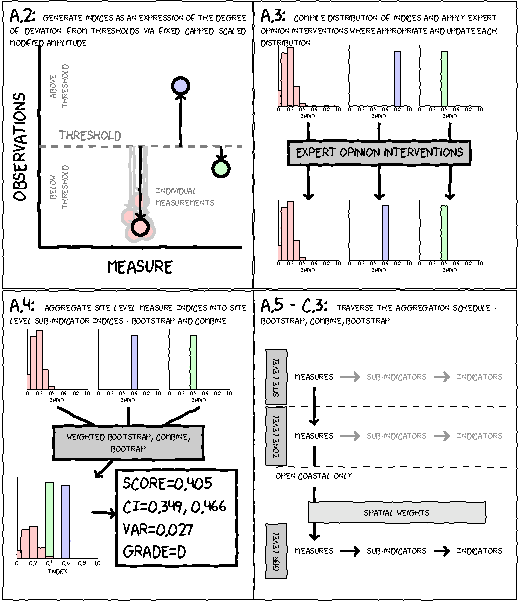
\includegraphics[width=\linewidth]{figures/Diagrams/schematic.pdf}
\caption[Schematic illustrating the major steps of the GBR Water Quality Report Card]{Schematic illustrating the major steps of the GBR Water Quality Report Card. In this fabricated example,
there are three Measures (Red, Green and Blue).  Each of the Blue and Green Measures are represented by a single
discrete observation, whereas the Red Measure is represented by a large collection of observations.
Expert option (top right panel) intervened to lower the blue Measure distribution from observed values at 0.8 to 0.6. Bootstrap aggregations (bottom left panel)
are used to combine data together proportionally.  Aggregation follows a specific pathway through the aggregation hierarchy depicted in the bottom right panel.
Great Barrier Reef (GBR) level aggregations utilize Open Coastal data only and aggregations are weighted according to proportional geographic areas of the Zones.
}\label{fig:schematic}
\end{figure}

\clearpage




\subsection{Aggregation summaries}

The ISP have indicated that the Water Quality metric should be based purely on eReefs fsMAMP indexed
Chlorophyll-a and Secchi Depth and that the conversion of scores to grades should follow a uniform
control chart.  Consequently, this section will only present graphical summaries for these metric
determinants.  %Other aggregation combinations can be found in Appendix~\ref{appsec:hierAgg}.

\subsubsection{Site/Measure level}

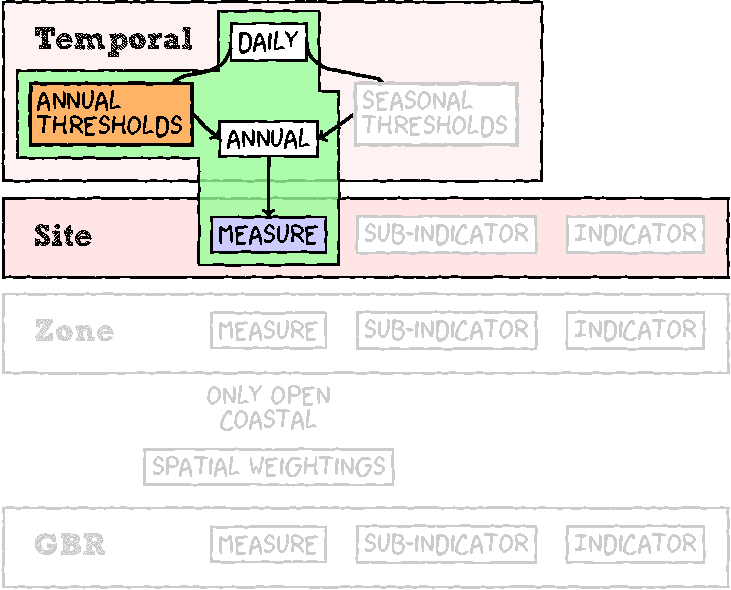
\includegraphics[width=0.5\linewidth]{{figures/Diagrams/hier_Site_Measure}.pdf}

\paragraph{Site level maps}

%Site/Measure (eReefs/fsMAMP/Uniform/chl) - spatial map
\begin{figure}[!hptb]
  \includegraphics[width=1\linewidth]{{figures/Indices/Maps/Measurement level/eReefs/spatial_map_eReefs_fsMAMP.Annual_measure.chl.site_Grade_Uniform\res}.png}
\caption{Spatio-temporal patterns in eReefs fsMAMP Chlorophyll-a index grades (Uniform grade type control chart applied).}\label{fig:spatial_map_eReefs_fsMAMP.Annual_measure.chl.site_Grade_Uniform_lowres}
\end{figure}

%Site/Measure (eReefs/fsMAMP/Uniform/sd) - spatial map
\begin{figure}[!hptb]
  \includegraphics[width=1\linewidth]{{figures/Indices/Maps/Measurement level/eReefs/spatial_map_eReefs_fsMAMP.Annual_measure.sd.site_Grade_Uniform\res}.png}
\caption{Spatio-temporal patterns in eReefs fsMAMP Secchi Depth index grades (Uniform grade type control chart applied).}\label{fig:spatial_map_eReefs_fsMAMP.Annual_measure.sd.site_Grade_Uniform_lowres}
\end{figure}

%\clearpage

\subsubsection{Site/Subindicator level}

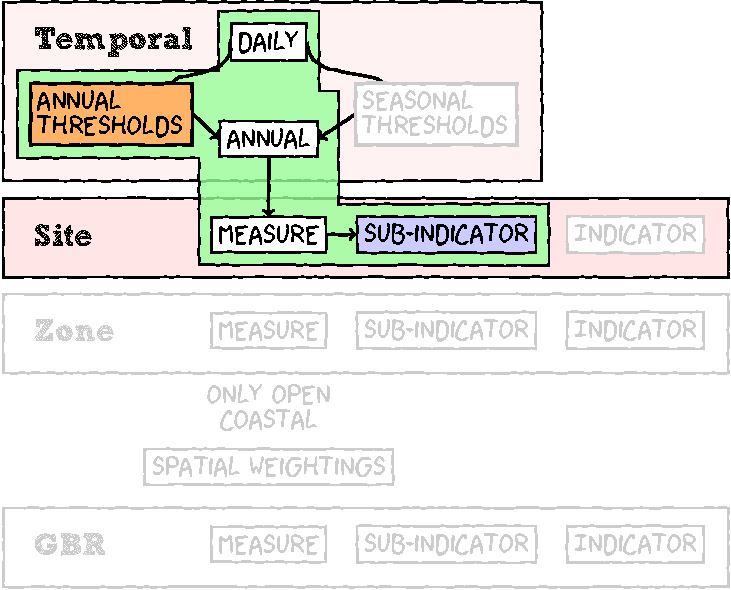
\includegraphics[width=0.5\linewidth]{{figures/Diagrams/hier_Site_Subindicator}.pdf}

\paragraph{Site level maps}

\begin{figure}[!hptb]
  \includegraphics[width=1\linewidth]{{figures/Indices/Maps/Subindicator level/eReefs/spatial_map_eReefs_fsMAMP.Annual_subindicator.Productivity.sitenoNOx_Grade_Uniform\res}.png}
\caption{Spatio-temporal patterns in eReefs fsMAMP Productivity index grades (Uniform grade type control chart applied).}\label{fig:spatial_map_eReefs_fsMAMP.Annual_subindictor.Productivity.sitenoNOx_Grade_Uniform_lowres}
\end{figure}

\begin{figure}[ptbh]
  \includegraphics[width=1\linewidth]{{figures/Indices/Maps/Subindicator level/eReefs/spatial_map_eReefs_fsMAMP.Annual_subindicator.Water Clarity.sitenoNOxnonap_Grade_Uniform\res}.png}
\caption{Spatio-temporal patterns in eReefs fsMAMP Water Clarity index grades (Uniform grade type control chart applied).}\label{fig:spatial_map_eReefs_fsMAMP.Annual_subindictor.Water Clarity.sitenoNOxnonap_Grade_Uniform_lowres}
\end{figure}


\subsubsection{Site/Indicator level}

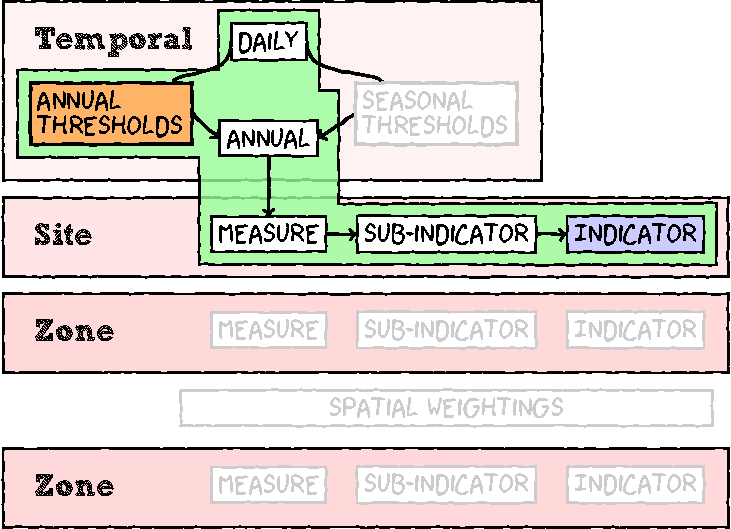
\includegraphics[width=0.5\linewidth]{{figures/Diagrams/hier_Site_Indicator}.pdf}

\paragraph{Site level maps}

\begin{figure}[ptbh]
  \includegraphics[width=1\linewidth]{{figures/Indices/Maps/Indicator level/eReefs/spatial_map_eReefs_fsMAMP.Annual_indicator.sitenoNOxnonap_A_Grade_Uniform\res}.png}
\caption{Spatio-temporal patterns in eReefs fsMAMP Water Quality index grades (Uniform grade type control chart applied).}\label{fig:spatial_map_eReefs_fsMAMP.Annual_indicator.sitenoNOxnonap_A_Grade_Uniform_lowres}
\end{figure}


       
\subsubsection{Zone/Measure level}

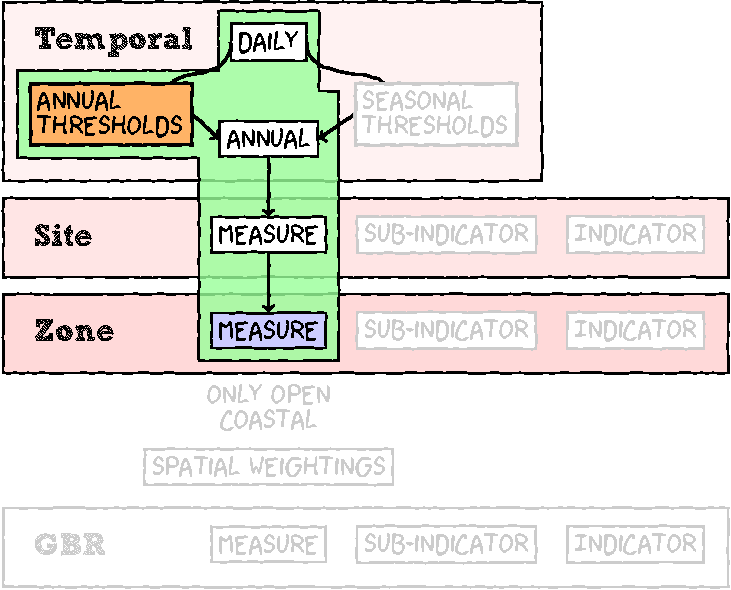
\includegraphics[width=0.5\linewidth]{{figures/Diagrams/hier_Zone_Measure}.pdf}

\paragraph{Simple time series}

\begin{figure}[!hptb]
  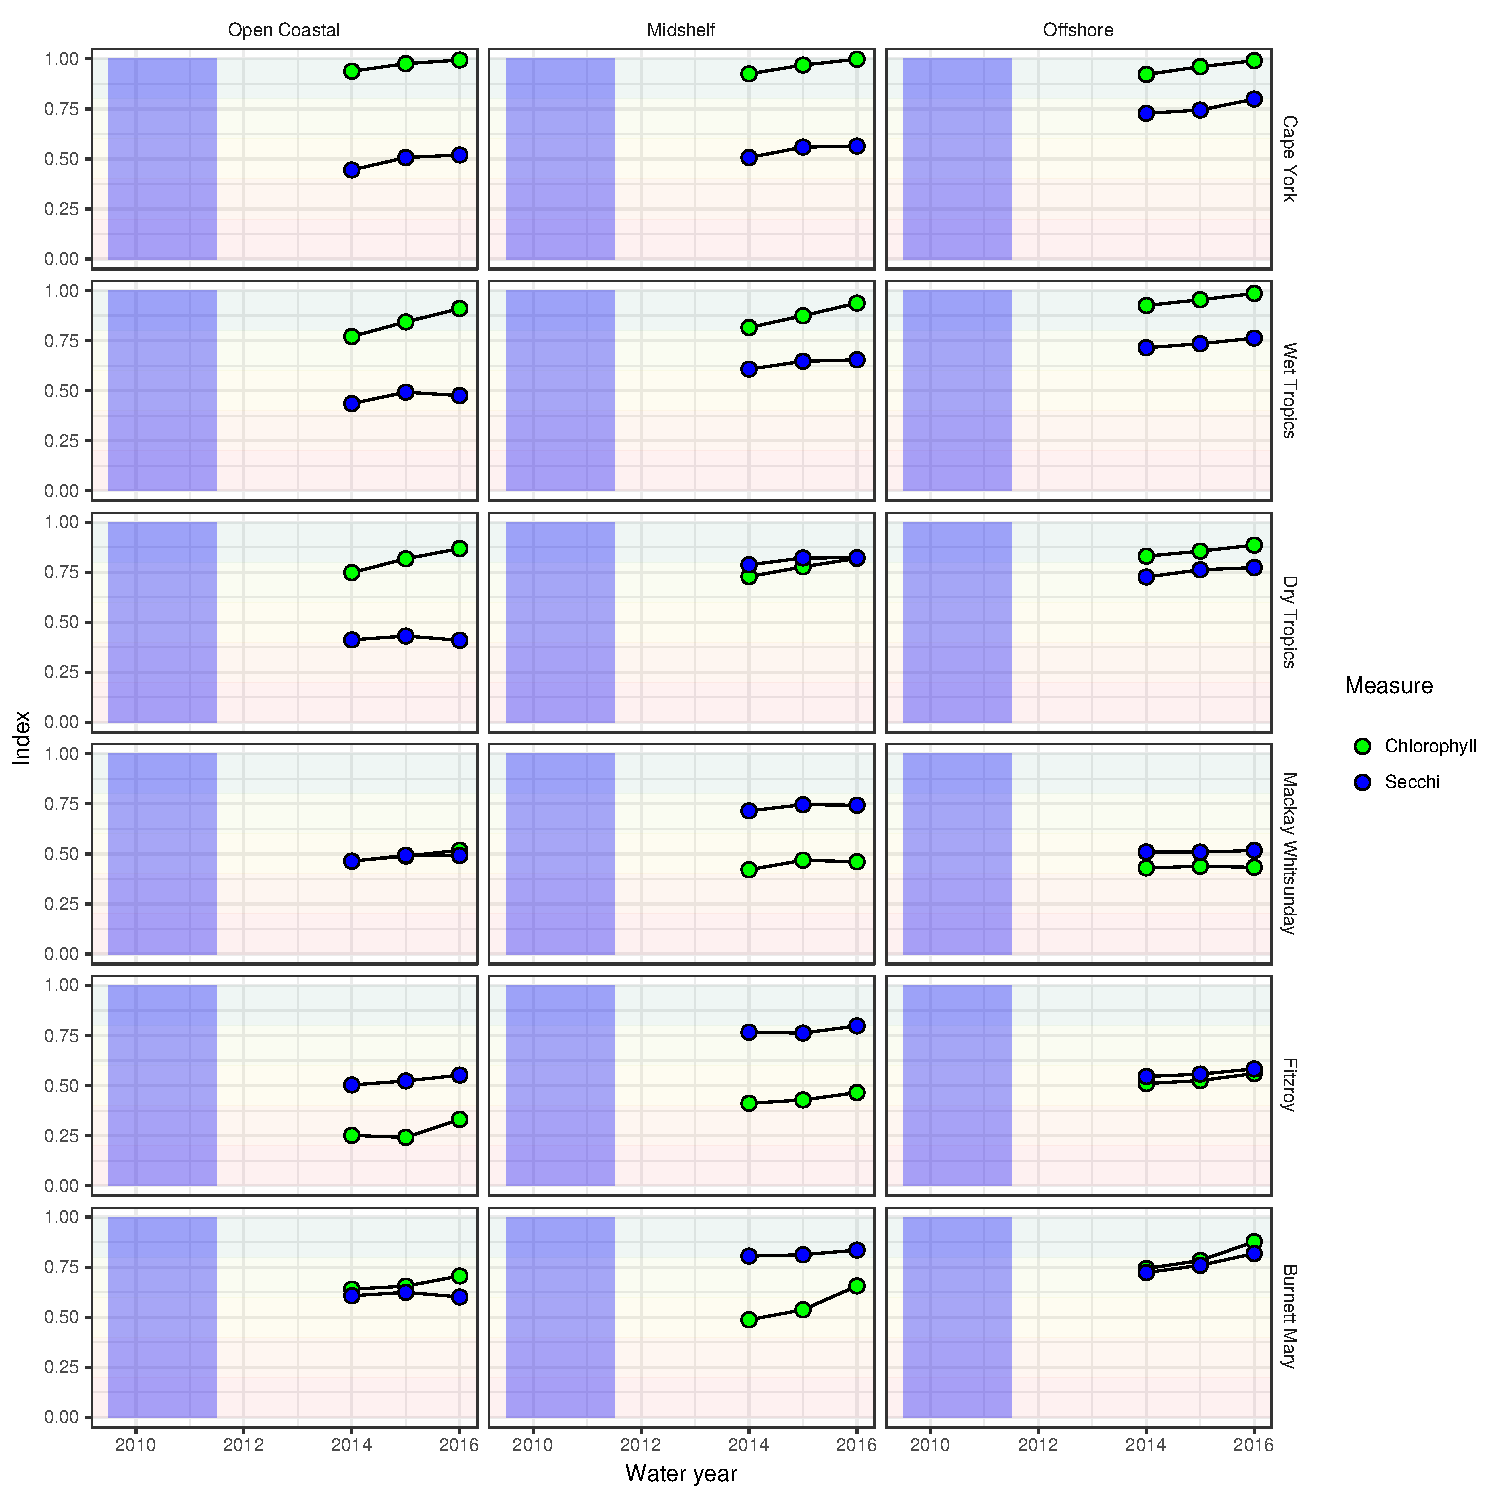
\includegraphics[width=1\linewidth]{{figures/Indices/Aggregations/eReefs/simple_eReefs_fsMAMP.Annual_measure.zonenoNOxnonap_without_enclosed_coastal_Grade_Uniform}.pdf}
\caption{Time series of fsMAMP measures (Chlorophyll-a and Secchi Depth) index scores by zone. The blue vertical bar spans from mid 2009 to mid 2011.  Faint colored horizontal bands represent Uniform grade ranges.}\label{fig:simple_eReefs_fsMAMP.Annual_measure.zonenoNOXnonap_with_enclosed_coastal_Grade_Uniform}
\end{figure}
\clearpage
 
\paragraph{Flat map}

\begin{figure}[ptbh]
  \includegraphics[width=1\linewidth]{{figures/Indices/Maps/Measurement level/eReefs/simple_map_eReefs_fsMAMP.Annual_measure_chl.zonenoNOxnonap_with_enclosed_coastal_A_Grade_Uniform\res}.png}
\caption{Simplified (Zone mean) eReefs spatio-temporal fsMAMP Chlorophyll-a index grades (Uniform grade type control chart applied).}\label{fig:simple_map_eReefs_fsMAMP.Annual_measure_chl.zonenoNOxnonap_with_enclosed_coastal_A_Grade_Uniform_lowres}
\end{figure}

%\begin{figure}[ptbh]
%  \includegraphics[width=1\linewidth]{{figures/Indices/Maps/Measurement level/eReefs/simple_map_eReefs_fsMAMP.Annual_measure_chl.zonenoSDnoNOXnonap_with_enclosed_coastal_A_Grade_MMP\res}.png}
%\caption{Simplified (Zone mean) eReefs spatio-temporal fsMAMP Chlorophyll-a index grades (MMP-like grade type control chart applied).}\label{fig:simple_map_eReefs_fsMAMP.Annual_measure_chl.zone_A_Grade_MMP_lowres}
%\end{figure}


%\begin{figure}[ptbh]
%  \includegraphics[width=1\linewidth]{{figures/Indices/Maps/Measurement level/eReefs/simple_map_eReefs_fsMAMP.Annual_measure_nap.zonenoNOxnonap_with_enclosed_coastal_A_Grade_Uniform\res}.png}
%\caption{Simplified (Zone mean) eReefs spatio-temporal fsMAMP TSS index grades (Uniform grade type control chart applied).}\label{fig:simple_map_eReefs_fsMAMP.Annual_measure_nap.zonenoNOXnonap_with_enclosed_coastal_A_Grade_Uniform_lowres}
%\end{figure}

%\begin{figure}[ptbh]
%  \includegraphics[width=1\linewidth]{{figures/Indices/Maps/Measurement level/eReefs/simple_map_eReefs_fsMAMP.Annual_measure_nap.zonenoSDnoNOxnonap_with_enclosed_coastal_A_Grade_MMP\res}.png}
%\caption{Simplified (Zone mean) eReefs spatio-temporal fsMAMP TSS index grades (MMP-like grade type control chart applied).}\label{fig:simple_map_eReefs_fsMAMP.Annual_measure_nap.zone_A_Grade_MMP_lowres}
%\end{figure}



\begin{figure}[ptbh]
  \includegraphics[width=1\linewidth]{{figures/Indices/Maps/Measurement level/eReefs/simple_map_eReefs_fsMAMP.Annual_measure_sd.zonenoNOxnonap_with_enclosed_coastal_A_Grade_Uniform\res}.png}
\caption{Simplified (Zone mean) eReefs spatio-temporal fsMAMP Secchi Depth index grades (Uniform grade type control chart applied).}\label{fig:simple_map_eReefs_fsMAMP.Annual_measure_sd.zonenoNOxnonap_with_enclosed_coastal_A_Grade_Uniform_lowres}
\end{figure}

%\begin{figure}[ptbh]
%  \includegraphics[width=1\linewidth]{{figures/Indices/Maps/Measurement level/eReefs/simple_map_eReefs_fsMAMP.Annual_measure_sd.zone_A_Grade_MMP\res}.png}
%\caption{Simplified (Zone mean) eReefs spatio-temporal fsMAMP Secchi Depth index grades (MMP-like grade type control chart applied).}\label{fig:simple_map_eReefs_fsMAMP.Annual_measure_sd.zone_A_Grade_MMP_lowres}
%\end{figure}
\clearpage

\paragraph{Mosaic plots level}
 
\begin{figure}[ptbh]
  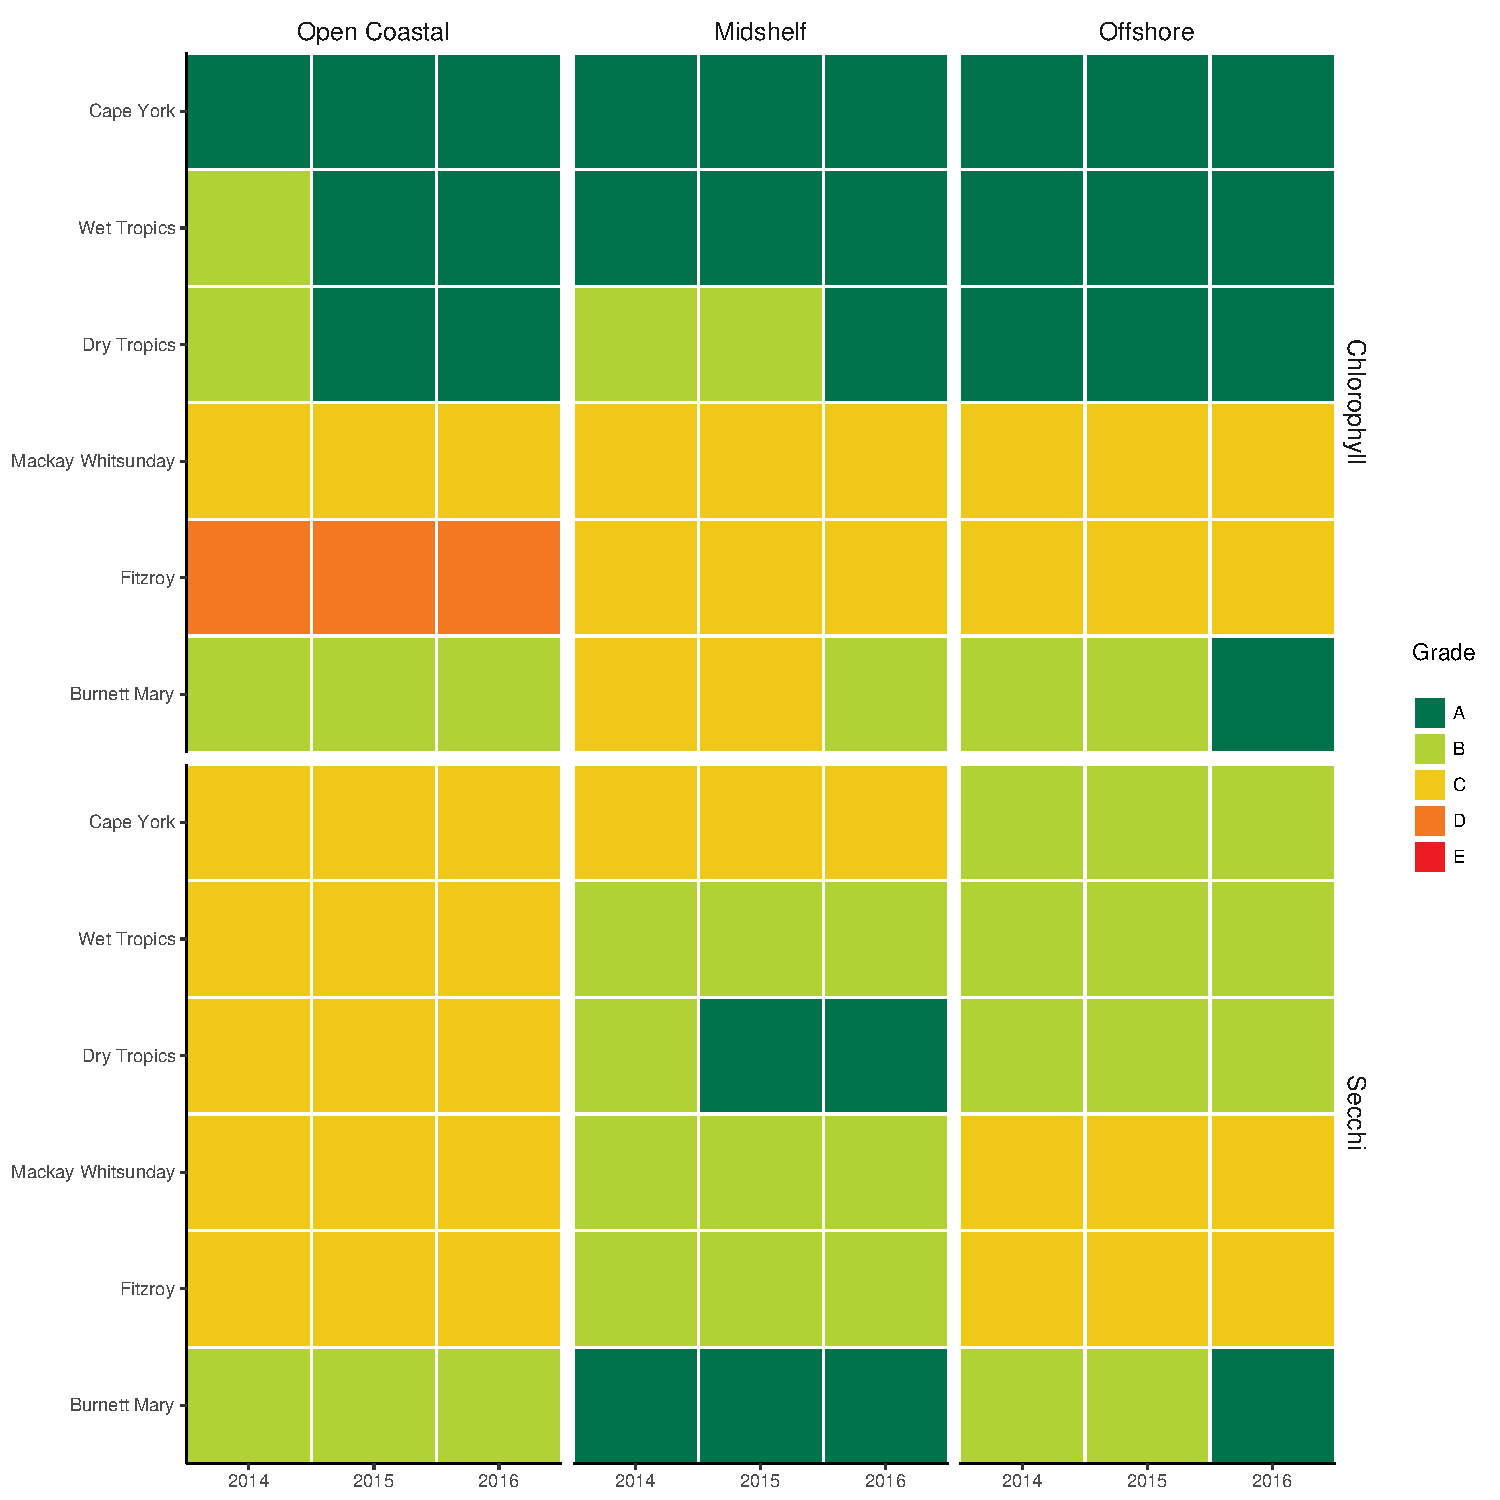
\includegraphics[width=1\linewidth]{{figures/Indices/Maps/Measurement level/eReefs/mosaic_eReefs_fsMAMP.Annual_measure.zonenoNOxnonap_without_enclosed_coastal_Grade_Uniform}.pdf}
\caption{Simplified (Zone mean) eReefs spatio-temporal fsMAMP Chlorophyll-a index grades (Uniform grade type control chart applied).}\label{fig:mosaic_eReefs_fsMAMP.Annual_measure.zonenoNOxnonap_with_enclosed_coastal_Grade_Uniform}
\end{figure}

%\begin{figure}[ptbh]
%  \includegraphics[width=1\linewidth]{{../Figures/Indices/Maps/Measurement level/eReefs/mosaic_eReefs_fsMAMP.Annual_measure.zone_Grade_MMP}.pdf}
%\caption{Simplified (Zone mean) eReefs spatio-temporal fsMAMP Chlorophyll-a index grades (Uniform grade type control chart applied).}\label{fig:mosaic_eReefs_fsMAMP.Annual_measure.zone_Grade_MMP}
%\end{figure}

\clearpage





\subsubsection{Zone/Subindicator}

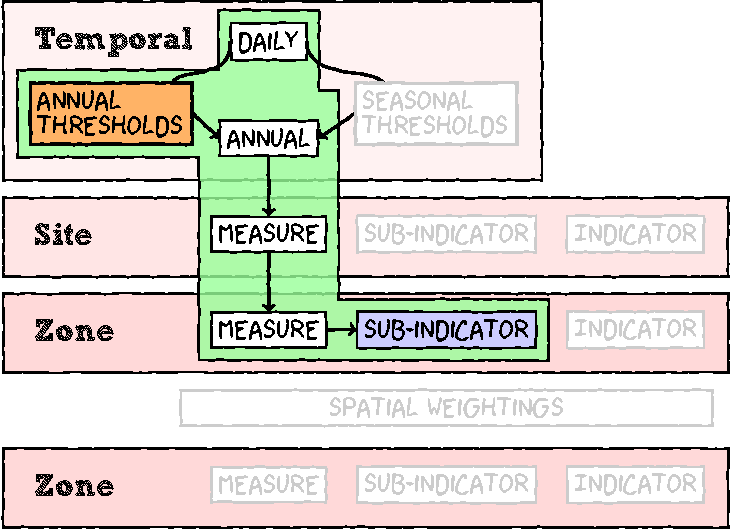
\includegraphics[width=0.5\linewidth]{{figures/Diagrams/hier_Zone_Subindicator}.pdf}

\paragraph{Simple time series}

\begin{figure}[ptbh]
  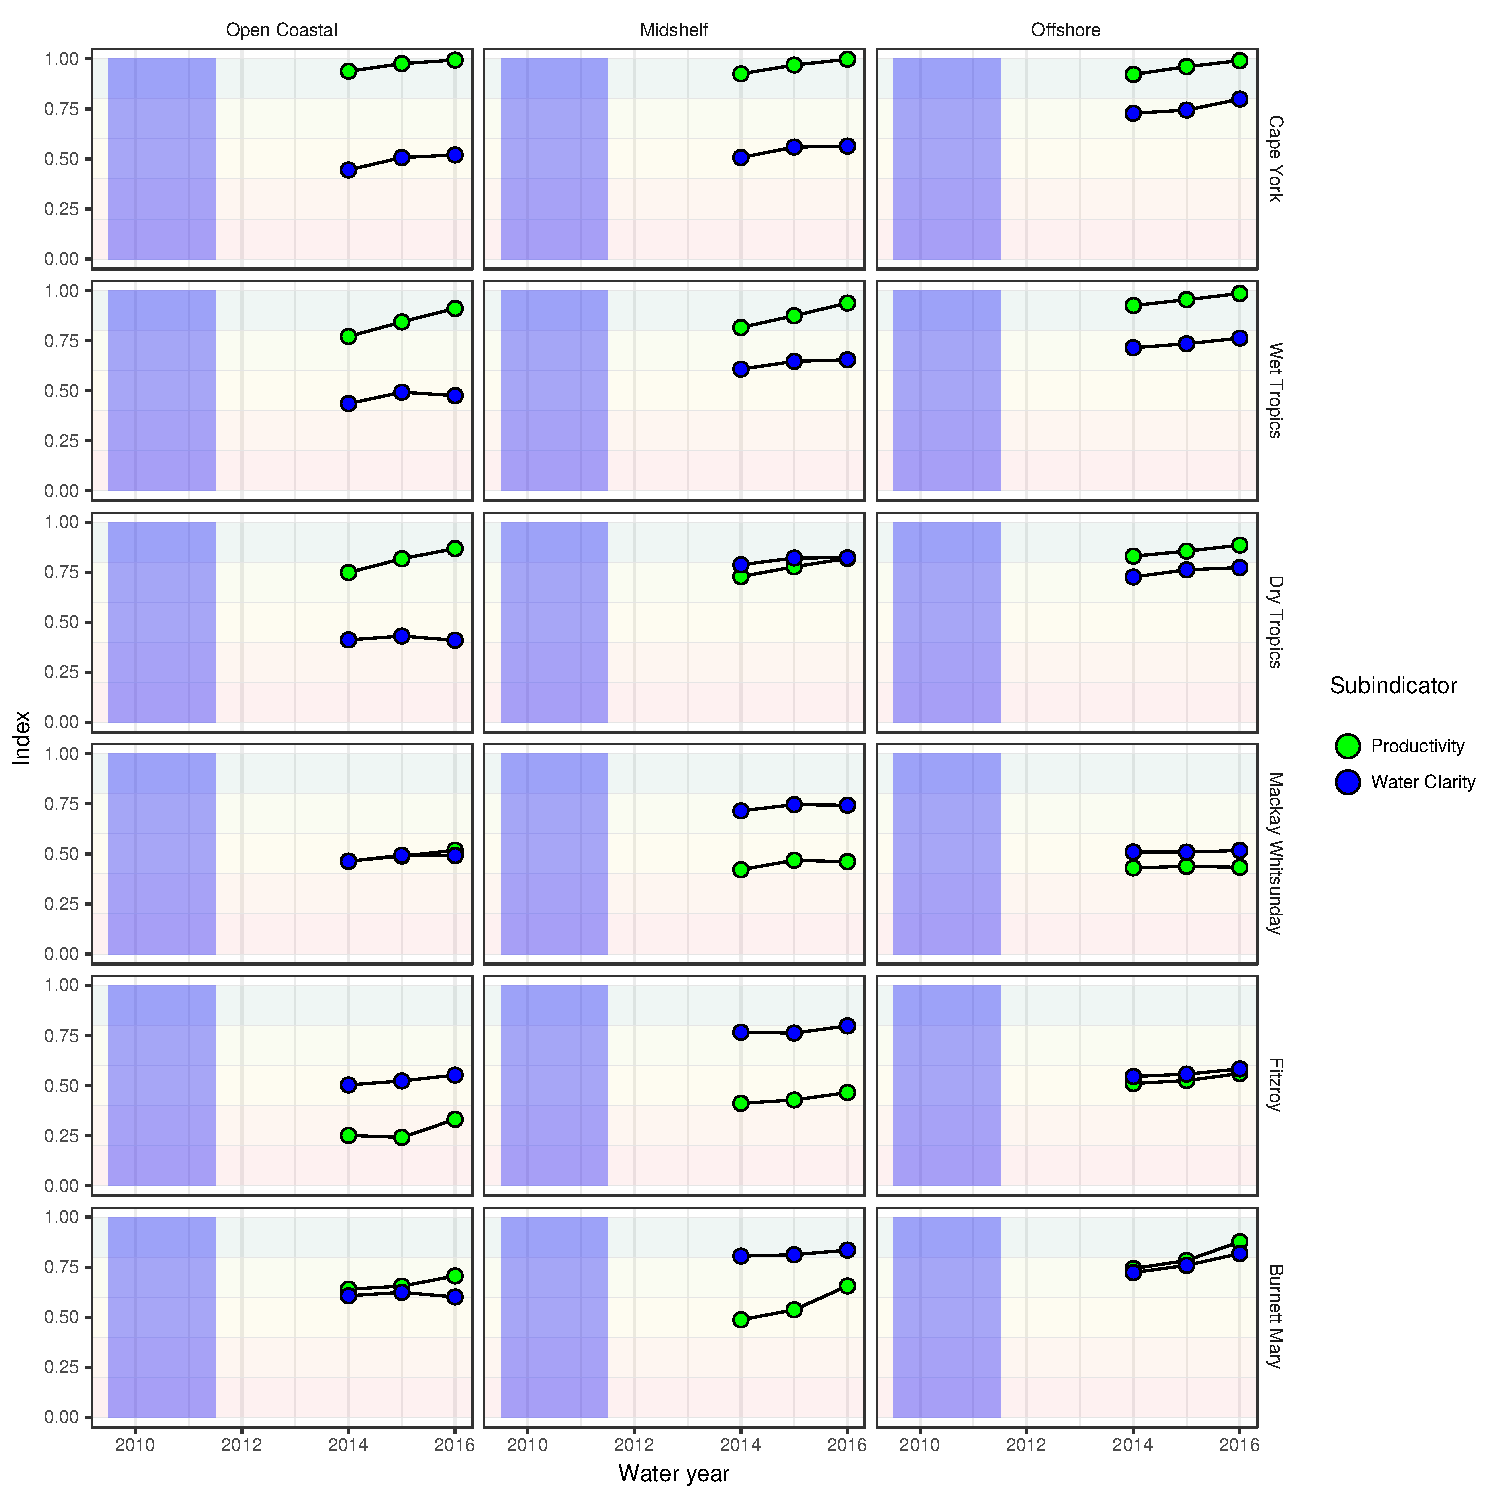
\includegraphics[width=1\linewidth]{{figures/Indices/Aggregations/eReefs/simple_eReefs_fsMAMP.Annual_subindicator.zonenoNOxnonap_without_enclosed_coastal_Grade_Uniform}.pdf}
\caption{Time series of fsMAMP Productivity and Water Clarity index scores by zone. The blue vertical bar spans from mid 2009 to mid 2011.  Faint colored horizontal bands represent Uniform grade ranges.}\label{fig:simple_eReefs_fsMAMP.Annual_subindicator.zonenoNOxnonap_Grade_Uniform}
\end{figure}
\clearpage

\paragraph{Flat map}

\begin{figure}[ptbh]
  \includegraphics[width=1\linewidth]{{figures/Indices/Maps/Subindicator level/eReefs/simple_map_eReefs_fsMAMP.Annual_subindicator_Productivity.zonenoNOxnonap_with_enclosed_coastal_A_Grade_Uniform\res}.png}
\caption{Simplified (Zone mean) eReefs spatio-temporal fsMAMP Productivity index grades (Uniform grade type control chart applied).}\label{fig:simple_map_eReefs_fsMAMP.Annual_subindicator_Productivity.zonenoNOxnonap_with_enclosed_coastal_A_Grade_Uniform_lowres}
\end{figure}

\begin{figure}[ptbh]
  \includegraphics[width=1\linewidth]{{figures/Indices/Maps/Subindicator level/eReefs/simple_map_eReefs_fsMAMP.Annual_subindicator_Water Clarity.zonenoNOxnonap_with_enclosed_coastal_A_Grade_Uniform\res}.png}
\caption{Simplified (Zone mean) eReefs spatio-temporal fsMAMP Water Clarity index grades (Uniform grade type control chart applied).}\label{fig:simple_map_eReefs_fsMAMP.Annual_subindicator_Water Clarity.zonenoNOxnonap_with_enclosed_coastal_A_Grade_Uniform_lowres}
\end{figure}


\paragraph{Mosaic plots}
  
\begin{figure}[ptbh]
  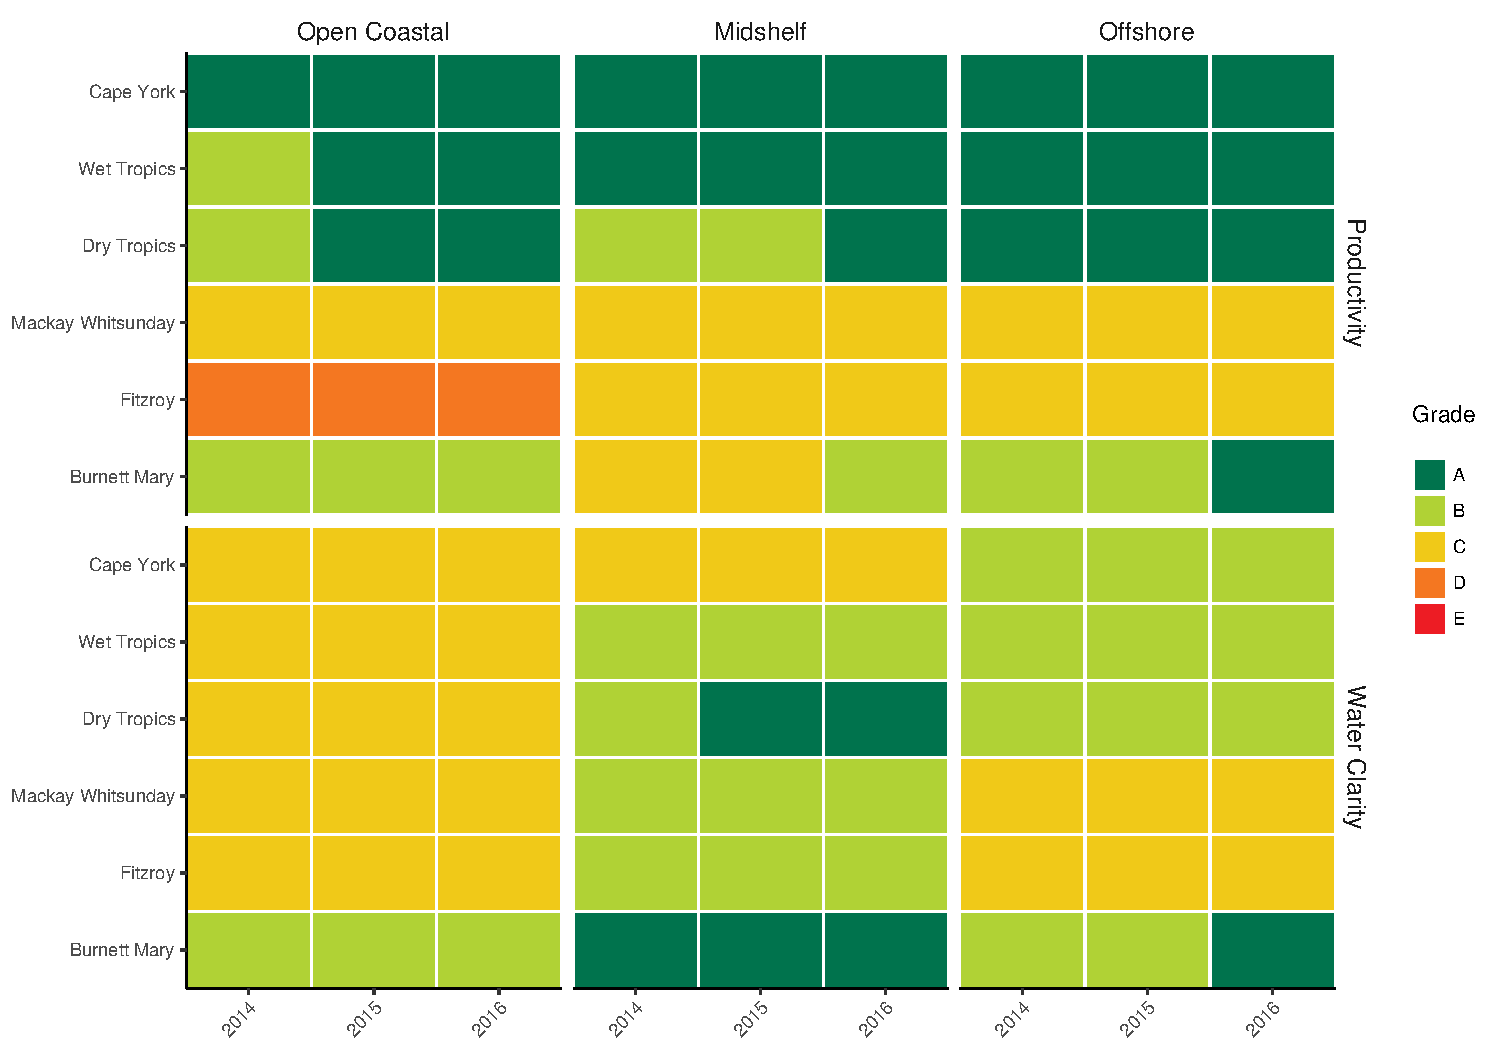
\includegraphics[width=1\linewidth]{{figures/Indices/Maps/Subindicator level/eReefs/mosaic_eReefs_fsMAMP.Annual_subindicator.zonenoNOxnonap_without_enclosed_coastal_Grade_Uniform}.pdf}
\caption{Simplified (Zone mean) eReefs spatio-temporal fsMAMP Subindicator index grades (Uniform grade type control chart applied).}\label{fig:mosaic_eReefs_fsMAMP.Annual_subindicator.zonenoNOxnonap_with_enclosed_coastal_Grade_Uniform}
\end{figure}

\clearpage


\subsubsection{Zone/Indicator level}

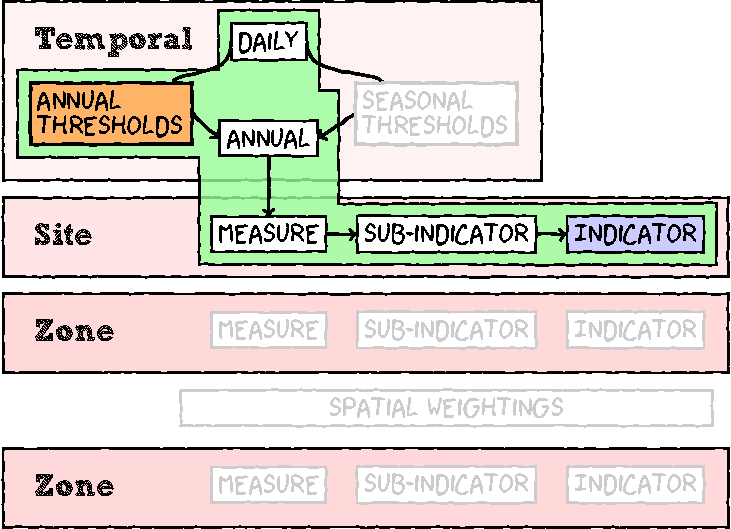
\includegraphics[width=0.5\linewidth]{{figures/Diagrams/hier_Site_Indicator}.pdf}

\paragraph{Simple time series}

\begin{figure}[ptbh]
  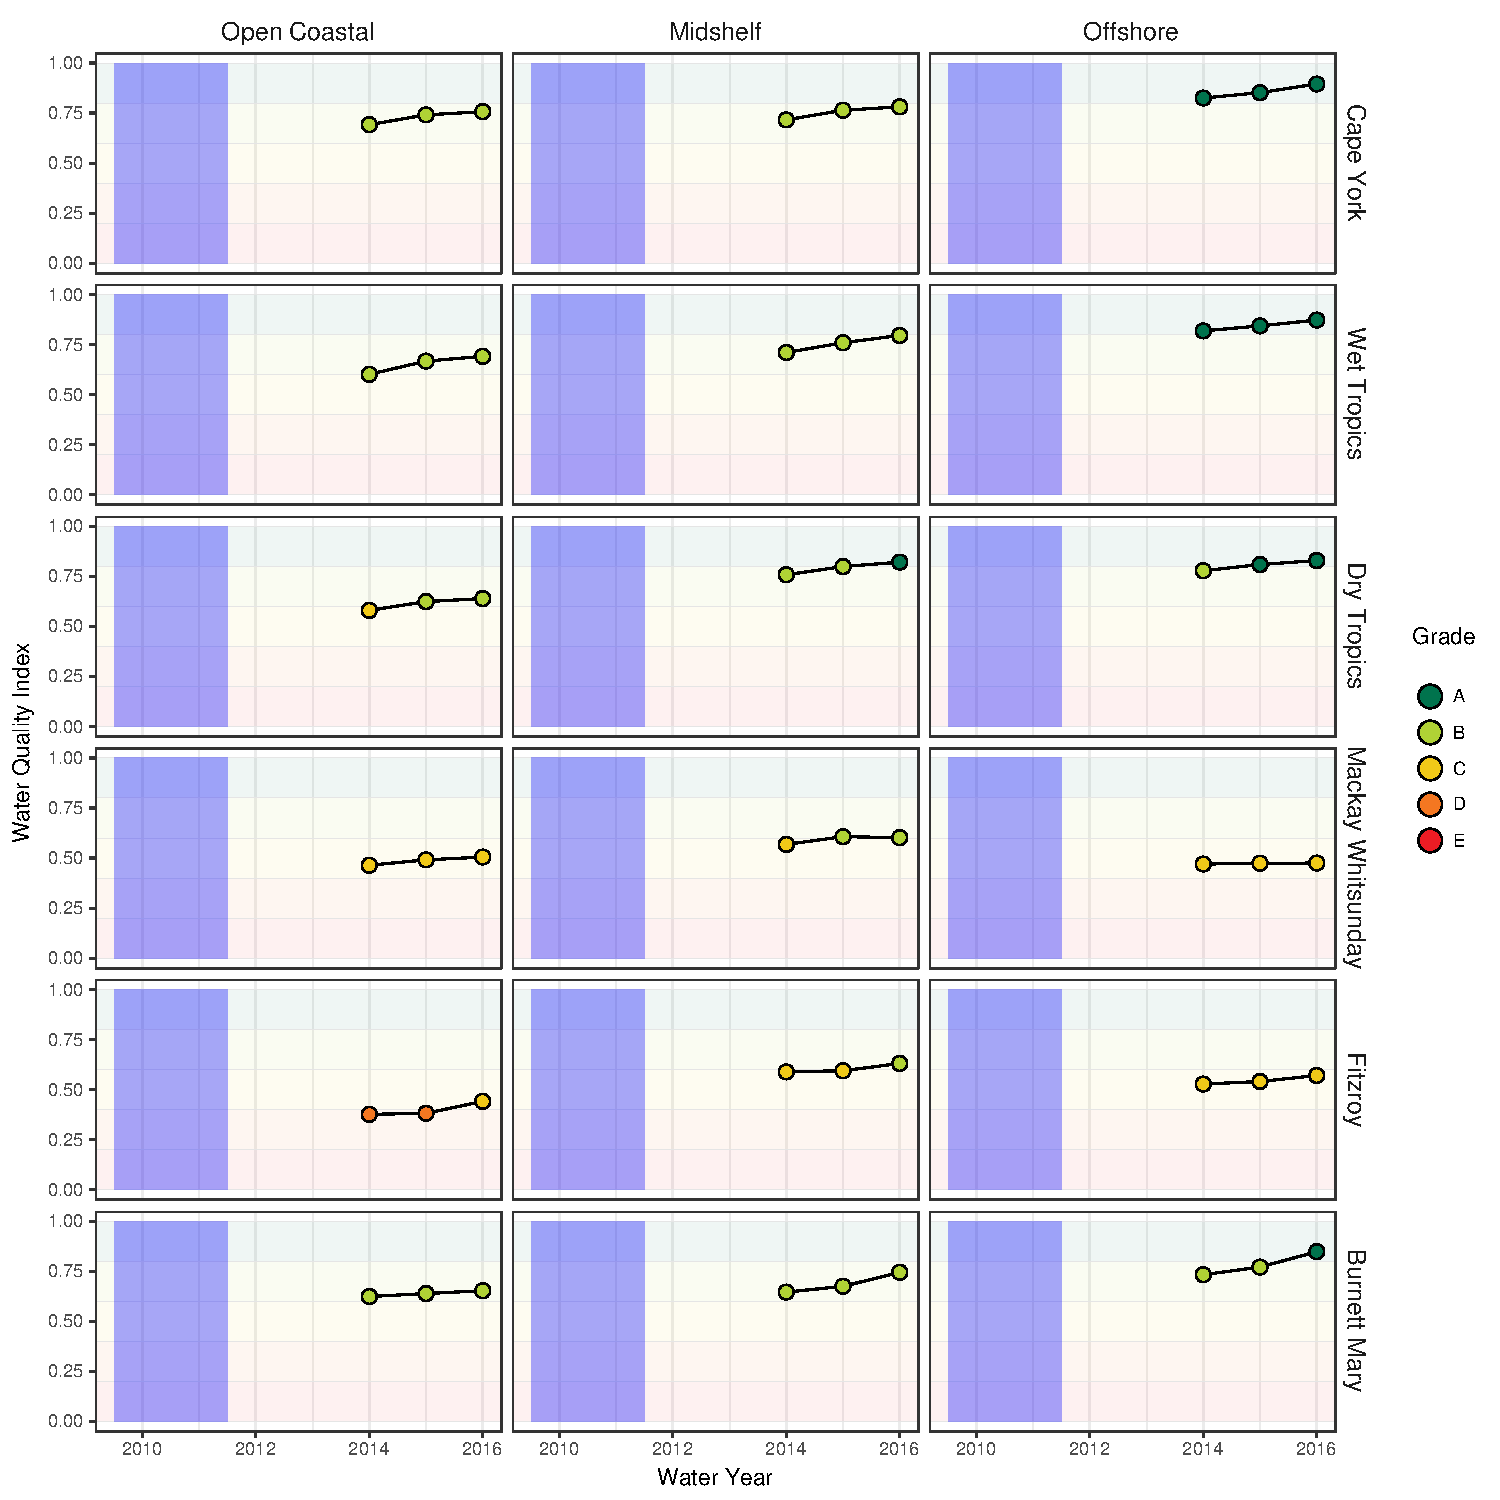
\includegraphics[width=1\linewidth]{{figures/Indices/Aggregations/eReefs/simple_eReefs_fsMAMP.Annual_indicator.zonenoNOxnonap_without_enclosed_coastal_A_Grade_Uniform}.pdf}
\caption{Time series of fsMAMP Water Quality index scores by zone. The blue vertical bar spans from mid 2009 to mid 2011.  Faint colored horizontal bands represent Uniform grade ranges.}\label{fig:simple_eReefs_fsMAMP.Annual_indicator.zonenoNOxnonap_with_enclosed_coastal_A_Grade_Uniform}
\end{figure}
\clearpage

\paragraph{Flat map}

\begin{figure}[ptbh]
  \includegraphics[width=1\linewidth]{{figures/Indices/Maps/Indicator level/eReefs/simple_map_eReefs_fsMAMP.Annual_indicator.zonenoNOxnonap_with_enclosed_coastal_A_Grade_Uniform\res}.png}
\caption{Simplified (Zone mean) eReefs spatio-temporal fsMAMP Productivity index grades (Uniform grade type control chart applied).}\label{fig:simple_map_eReefs_fsMAMP.Annual_indicator.sitenoNOxnonap_with_enclosed_coastal_A_Grade_Uniform_lowres}
\end{figure}

\paragraph{Mosaic plots}
  
\begin{figure}[ptbh]
  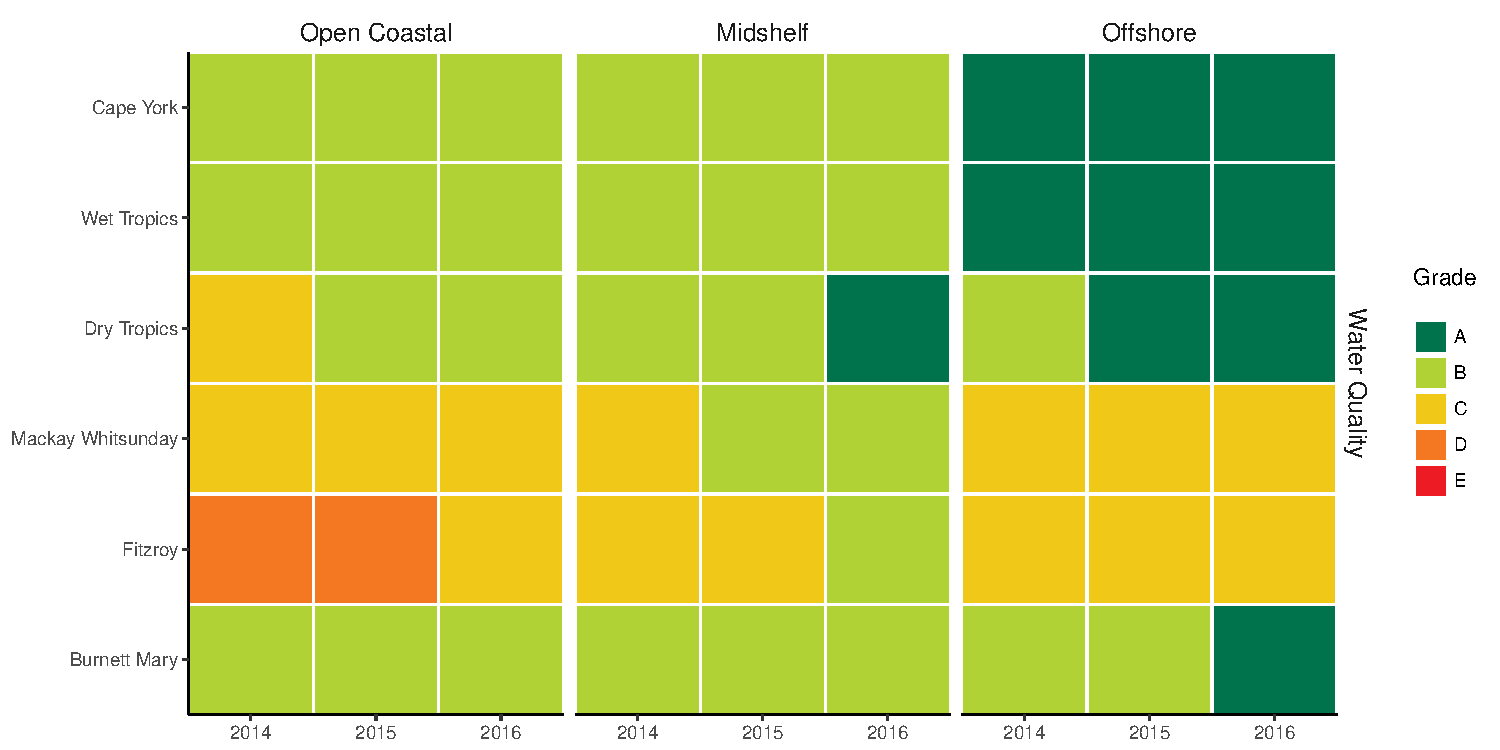
\includegraphics[width=1\linewidth]{{figures/Indices/Maps/Indicator level/eReefs/mosaic_eReefs_fsMAMP.Annual_indicator.zonenoNOxnonap_without_enclosed_coastal_Grade_Uniform}.pdf}
\caption{Simplified (Zone mean) eReefs spatio-temporal fsMAMP indicator index grades (Uniform grade type control chart applied).}\label{fig:mosaic_eReefs_fsMAMP.Annual_indicator.zonenoNOxnonap_with_enclosed_coastal_Grade_Uniform}
\end{figure}


%\begin{figure}[ptbh]
%  \includegraphics[width=1\linewidth]{{figures/Indices/Maps/Indicator level/Satellite/spatial_map__fsMAMP.Annual_indicator.sitenoSDnoNOxnonap_A\res}.pdf}
%\caption{Spatio-temporal Satellite fsMAMP Water Quality index scores for each data source.}\label{fig:spatial_map__fsMAMP.Annual_indicator.sitenoSDnoNOxnonap_A}
%\end{figure}
 
%\begin{figure}[ptbh]
%  \includegraphics[width=1\linewidth]{{figures/Indices/Maps/Indicator level/eReefs/spatial_map_eReefs_fsMAMP.Annual_indicator.sitenoNOxnonap_A_Grade_Uniform}.pdf}
%  \caption{Spatio-temporal eReefs fsMAMP Water Quality index scores for each data source.}\label{fig:spatial_map_eReefs_fsMAMP.Annual_indicator.sitenoSDnoNOxnonap_A}
%\end{figure}
 
%\begin{figure}[ptbh]
%  \includegraphics[width=1\linewidth]{{../Figures/Indices/Maps/Indicator level/eReefs926/spatial_map_eReefs926_fsMAMP.Annual_indicator.sitenoSDnoNOxnonap_A\res}.pdf}
%  \caption{Spatio-temporal eReefs926 fsMAMP Water Quality index scores for each data source.}\label{fig:spatial_map_eReefs926_fsMAMP.Annual_indicator.sitenoSDnoNOxnonap_A}
%\end{figure}


\clearpage





% \subsubsection{Indicator/Zone}
% \begin{figure}[ptbh]
%   \includegraphics[width=1\linewidth]{{../Figures/Indices/Aggregations/Satellite/simple__fsMAMP.Annual_indicator.zonenoSDnoNOx_A}.pdf}
%   \caption{Time series of Satellite fsMAMP Water Quality Index grades by zone. The blue vertical bar spans from mid 2009 to mid 2011.}\label{fig:simple__fsMAMP.Annual_indicator.zonenoSDnoNOx_A}
% \end{figure}

% \begin{figure}[ptbh]
%   \includegraphics[width=1\linewidth]{{../Figures/Indices/Aggregations/eReefs/simple_eReefs_fsMAMP.Annual_indicator.zonenoSDnoNOx_A}.pdf}
% \caption{Time series of eReefs fsMAMP Water Quality index scores by zone. The blue vertical bar spans from mid 2009 to mid 2011.}\label{fig:simple_eReefs_fsMAMP.Annual_indicator.zonenoSDnoNOx_A}
% \end{figure}

% \begin{figure}[ptbh]
%   \includegraphics[width=1\linewidth]{{../Figures/Indices/Aggregations/eReefs926/simple_eReefs926_fsMAMP.Annual_indicator.zonenoSDnoNOx_A}.pdf}
% \caption{Time series of eReefs926 fsMAMP Water Quality index scores by zone. The blue vertical bar spans from mid 2009 to mid 2011.}\label{fig:simple_eReefs926_fsMAMP.Annual_indicator.zonenoSDnoNOx_A}
% \end{figure}
% \clearpage

% \begin{figure}[ptbh] 
%   \includegraphics[width=1\linewidth]{{../Figures/Indices/Maps/Indicator level/Satellite/simple_map__fsMAMP.Annual_indicator.zonenoSDnoNOx_A\res}.pdf}
% \caption{Simplified (Zone mean) Satellite spatio-temporal fsMAMP Water Quality index scores.}\label{fig:simple_map__fsMAMP.Annual_indicator.zonenoSDnoNOx_A}
% \end{figure} 

% \begin{figure}[ptbh] 
%   \includegraphics[width=1\linewidth]{{../Figures/Indices/Maps/Indicator level/eReefs/simple_map_eReefs_fsMAMP.Annual_indicator.zonenoSDnoNOx_A\res}.pdf}
% \caption{Simplified (Zone mean) eReefs spatio-temporal fsMAMP Water Quality index scores.}\label{fig:simple_map_eReefs_fsMAMP.Annual_indicator.zonenoSDnoNOx_A}
% \end{figure}  

% \begin{figure}[ptbh] 
%   \includegraphics[width=1\linewidth]{{../Figures/Indices/Maps/Indicator level/eReefs926/simple_map_eReefs926_fsMAMP.Annual_indicator.zonenoSDnoNOx_A\res}.pdf}
%   \caption{Simplified (Zone mean) eReefs926 spatio-temporal fsMAMP Water Quality index scores.}\label{fig:simple_map_eReefs926_fsMAMP.Annual_indicator.zonenoSDnoNOx_A}
% \end{figure} 
  
% \clearpage

% \begin{figure}[ptbh]
%   \includegraphics[width=1\linewidth]{{../Figures/Indices/Maps/Indicator level/Satellite/mosaic__fsMAMP.Annual_indicator.zonenoSDnoNOx}.pdf}
% \caption{Time series of Satellite fsMAMP Water Quality index scores by zone}\label{fig:mosaic__fsMAMP.Annual_indicator.zonenoSDnoNOx}
% \end{figure}

% \begin{figure}[ptbh]
%   \includegraphics[width=1\linewidth]{{../Figures/Indices/Maps/Indicator level/eReefs/mosaic_eReefs_fsMAMP.Annual_indicator.zonenoSDnoNOx}.pdf}
% \caption{Time series of eReefs fsMAMP Water Quality index scores by zone}\label{fig:mosaic_eReefs_fsMAMP.Annual_indicator.zonenoSDnoNOx}
% \end{figure}

% \begin{figure}[ptbh]
%   \includegraphics[width=1\linewidth]{{../Figures/Indices/Maps/Indicator level/eReefs926/mosaic_eReefs926_fsMAMP.Annual_indicator.zonenoSDnoNOx}.pdf}
% \caption{Time series of eReefs926 fsMAMP Water Quality index scores by zone}\label{fig:mosaic_eReefs926_fsMAMP.Annual_indicator.zonenoSDnoNOx}
% \end{figure}
 
\clearpage


%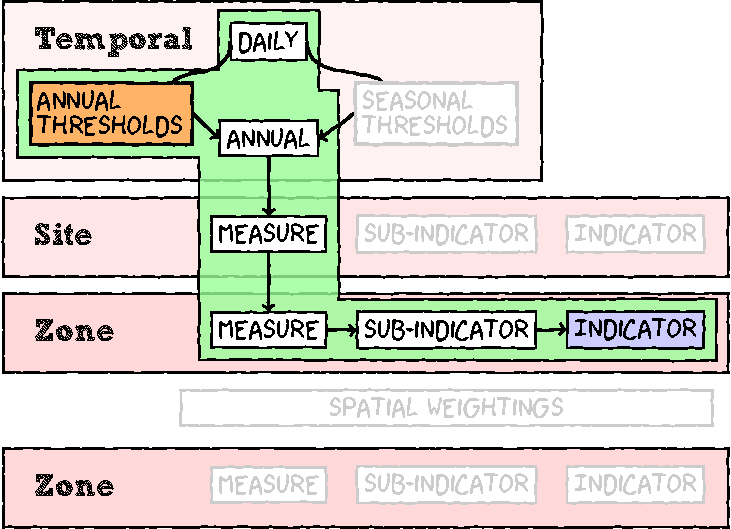
\includegraphics[width=0.5\linewidth]{{figures/Diagrams/hier_Zone_Indicator}.pdf}
%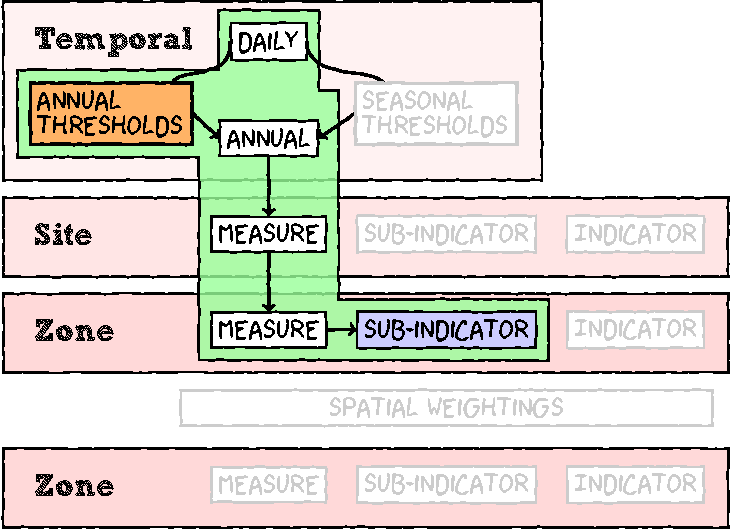
\includegraphics[width=0.5\linewidth]{{figures/Diagrams/hier_Zone_Subindicator}.pdf}



%\includegraphics[width=0.5\linewidth]{{figures/Diagrams/hier_GBR_Indicator}.pdf}
%\includegraphics[width=0.5\linewidth]{{figures/Diagrams/hier_GBR_Subindicator}.pdf}
%\includegraphics[width=0.5\linewidth]{{figures/Diagrams/hier_GBR_Measure}.pdf}


\subsection{Aggregations to water body level}

\subsubsection{Water body/Measure level}

\includegraphics[width=0.5\linewidth]{{figures/Diagrams/hier_GBR_Measure}.pdf}

\paragraph{Simple time series}

\begin{figure}[ptbh]
  \includegraphics[width=1\linewidth]{{figures/Indices/Aggregations/eReefs/simple_eReefs_fsMAMP.Annual_measure.waterbodynoNOxnonap_without_enclosed_coastal_Grade_Uniform}.pdf}
\caption{Time series of fsMAMP Measure index scores by water body (aggregated over management region weighted by area). The blue vertical bar spans from mid 2009 to mid 2011.  Faint colored horizontal bands represent Uniform grade ranges.}\label{fig:simple_eReefs_fsMAMP.Annual_measure.waterbodynoNOx_with_enclosed_coastal_Grade_Uniform}
\end{figure}
\clearpage

\paragraph{Mosaic plots}
  
\begin{figure}[!hptb]
  \includegraphics[width=1\linewidth]{{figures/Indices/Maps/Measurement level/eReefs/mosaic_eReefs_fsMAMP.Annual_measure.waterbodynoNOxnonap_without_enclosed_coastal_Grade_Uniform}.pdf}
\caption{Simplified (Zone mean) eReefs spatio-temporal fsMAMP Measurement index grades (Uniform grade type control chart applied).}\label{fig:mosaic_eReefs_fsMAMP.Annual_measure.waterbodynoNOxnonap_with_enclosed_coastal_Grade_Uniform}
\end{figure}



\subsubsection{Water body/Subindicator level}

\includegraphics[width=0.5\linewidth]{{figures/Diagrams/hier_GBR_Subindicator}.pdf}

\paragraph{Simple time series}

\begin{figure}[!hptb]
  \includegraphics[width=1\linewidth]{{figures/Indices/Aggregations/eReefs/simple_eReefs_fsMAMP.Annual_subindicator.waterbodynoNOxnonap_without_enclosed_coastal_Grade_Uniform}.pdf}
\caption{Time series of fsMAMP Subindicator index scores by water body (aggregated over management region weighted by area). The blue vertical bar spans from mid 2009 to mid 2011.  Faint colored horizontal bands represent Uniform grade ranges.}\label{fig:simple_eReefs_fsMAMP.Annual_subindicator.waterbodynoNOx_with_enclosed_coastal_Grade_Uniform}
\end{figure}
\clearpage

\paragraph{Mosaic plots}
  
\begin{figure}[!hptb]
  \includegraphics[width=1\linewidth]{{figures/Indices/Maps/Subindicator level/eReefs/mosaic_eReefs_fsMAMP.Annual_subindicator.waterbodynoNOxnonap_without_enclosed_coastal_Grade_Uniform}.pdf}
\caption{Simplified (Zone mean) eReefs spatio-temporal fsMAMP Subindicator index grades (Uniform grade type control chart applied).}\label{fig:mosaic_eReefs_fsMAMP.Annual_subindicator.waterbodynoNOx_with_enclosed_coastal_Grade_Uniform}
\end{figure}


\subsubsection{Water body/Indicator level}

\includegraphics[width=0.5\linewidth]{{figures/Diagrams/hier_GBR_Indicator}.pdf}

\paragraph{Simple time series}

\begin{figure}[ptbh]
  \includegraphics[width=1\linewidth]{{figures/Indices/Aggregations/eReefs/simple_eReefs_fsMAMP.Annual_indicator.waterbodynoNOx_without_enclosed_coastal_Grade_Uniform}.pdf}
\caption{Time series of fsMAMP Indicator index scores by water body (aggregated over management region weighted by area). The blue vertical bar spans from mid 2009 to mid 2011.  Faint colored horizontal bands represent Uniform grade ranges.}\label{fig:simple_eReefs_fsMAMP.Annual_indicator.waterbodynoNOx_with_enclosed_coastal_Grade_Uniform}
\end{figure}
\clearpage

\paragraph{Mosaic plots}
  
\begin{figure}[ptbh]
  \includegraphics[width=1\linewidth]{{figures/Indices/Maps/Indicator level/eReefs/mosaic_eReefs_fsMAMP.Annual_indicator.waterbodynoNOx_without_enclosed_coastal_Grade_Uniform}.pdf}
\caption{Simplified (Zone mean) eReefs spatio-temporal fsMAMP Indicator index grades (Uniform grade type control chart applied).}\label{fig:mosaic_eReefs_fsMAMP.Annual_indicator.waterbodynoNOx_with_enclosed_coastal_Grade_Uniform}
\end{figure}



\subsection{Aggregations to GBR level}

\subsubsection{GBR/Measure level}

\includegraphics[width=0.5\linewidth]{{figures/Diagrams/hier_GBR_Measure}.pdf}

\paragraph{Simple time series}

\begin{figure}[ptbh]
  \includegraphics[width=1\linewidth]{{figures/Indices/Aggregations/eReefs/simple_eReefs_fsMAMP.Annual_measure.gbrnoNOxnonap_with_enclosed_coastal_Grade_Uniform}.pdf}
\caption{Time series of fsMAMP Measure index scores by GBR (aggregated over management region weighted by area). The blue vertical bar spans from mid 2009 to mid 2011.  Faint colored horizontal bands represent Uniform grade ranges.}\label{fig:simple_eReefs_fsMAMP.Annual_measure.gbrnoNOx_with_enclosed_coastal_Grade_Uniform}
\end{figure}
\clearpage

\paragraph{Mosaic plots}
  
\begin{figure}[ptbh]
  \includegraphics[width=1\linewidth]{{figures/Indices/Maps/Measurement level/eReefs/mosaic_eReefs_fsMAMP.Annual_measure.gbrnoNOxnonap_with_enclosed_coastal_Grade_Uniform}.pdf}
\caption{Simplified (Zone mean) eReefs spatio-temporal fsMAMP Measurement index grades (Uniform grade type control chart applied).}\label{fig:mosaic_eReefs_fsMAMP.Annual_measure.gbrnoNOx_with_enclosed_coastal_Grade_Uniform}
\end{figure}



\subsubsection{GBR/Subindicator level}

\includegraphics[width=0.5\linewidth]{{figures/Diagrams/hier_GBR_Subindicator}.pdf}

\paragraph{Simple time series}

\begin{figure}[ptbh]
  \includegraphics[width=1\linewidth]{{figures/Indices/Aggregations/eReefs/simple_eReefs_fsMAMP.Annual_subindicator.gbrnoNOxnonap_with_enclosed_coastal_Grade_Uniform}.pdf}
\caption{Time series of fsMAMP Subindicator index scores by GBR (aggregated over management region weighted by area). The blue vertical bar spans from mid 2009 to mid 2011.  Faint colored horizontal bands represent Uniform grade ranges.}\label{fig:simple_eReefs_fsMAMP.Annual_subindicator.gbrnoNOx_with_enclosed_coastal_Grade_Uniform}
\end{figure}
\clearpage

\paragraph{Mosaic plots}
  
\begin{figure}[ptbh]
  \includegraphics[width=1\linewidth]{{figures/Indices/Maps/Subindicator level/eReefs/mosaic_eReefs_fsMAMP.Annual_subindicator.gbrnoNOxnonap_with_enclosed_coastal_Grade_Uniform}.pdf}
\caption{Simplified (Zone mean) eReefs spatio-temporal fsMAMP Subindicator index grades (Uniform grade type control chart applied).}\label{fig:mosaic_eReefs_fsMAMP.Annual_subindicator.gbrnoNOx_with_enclosed_coastal_Grade_Uniform}
\end{figure}


\subsubsection{GBR/Indicator level}

\includegraphics[width=0.5\linewidth]{{figures/Diagrams/hier_GBR_Indicator}.pdf}

\paragraph{Simple time series}

\begin{figure}[ptbh]
  \includegraphics[width=1\linewidth]{{figures/Indices/Aggregations/eReefs/simple_eReefs_fsMAMP.Annual_indicator.gbrnoNOxnonap_with_enclosed_coastal_Grade_Uniform}.pdf}
\caption{Time series of fsMAMP Indicator index scores by GBR (aggregated over management region weighted by area). The blue vertical bar spans from mid 2009 to mid 2011.  Faint colored horizontal bands represent Uniform grade ranges.}\label{fig:simple_eReefs_fsMAMP.Annual_indicator.gbrnoNOx_with_enclosed_coastal_Grade_Uniform}
\end{figure}
\clearpage

\paragraph{Mosaic plots}
  
\begin{figure}[ptbh]
  \includegraphics[width=1\linewidth]{{figures/Indices/Maps/Indicator level/eReefs/mosaic_eReefs_fsMAMP.Annual_indicator.gbrnoNOxnonap_with_enclosed_coastal_Grade_Uniform}.pdf}
\caption{Simplified (Zone mean) eReefs spatio-temporal fsMAMP Indicator index grades (Uniform grade type control chart applied).}\label{fig:mosaic_eReefs_fsMAMP.Annual_indicator.gbrnoNOx_with_enclosed_coastal_Grade_Uniform}
\end{figure}



% Compare Measures aggregated to Zone level

% - dependent on selection of sources etc..
 

\subsection{Summary of recommendations}


\begin{minipage}[t]{\textwidth}
\textbf{A. Calculation of Zone level Score and Grades}
\begin{enumerate}
\item Collect raw data (= \textbf{Measures}) for Chlorophyll-a and Secchi depth at each fixed monitoring site and compare individual observations to associated threshold/benchmark/reference or set of expectation ranges
\item Create indexed data as an expression of degree of difference (\textit{scaled modified amplitude method}) to yield a \textbf{Score} for each \textbf{Measure} (Chlorophyll-a and Secchi depth) per sampling location (e.g. Site)
\item Combine \textbf{Measure} Scores into \textbf{Site}-level \textbf{Sub-indicator} (Productivity and Water Clarity) Scores by averaging  
\item Combine \textbf{Sub-indicator} Scores into \textbf{Site}-level \textbf{Indicator} (Water Quality) Scores by averaging.
\item Convert Scores into coloured \textbf{Grades} (A-E) for visual presentation in report card
\end{enumerate}
\textbf{B.     Calculation of Zone level Grades}
\begin{enumerate}
\item Aggregate \textbf{Site}-level \textit{Measure} Scores from step A.1 into \textbf{Zone}-level \textit{Measure} Scores by averaging.
\item Aggregate \textbf{Zone}-level \textit{Measure} Scores into \textbf{Zone}-level \textit{Subindicator} Scores by averaging.
\item Aggregate \textbf{Zone}-level \textit{Subindicator} Scores into \textbf{Zone}-level \textit{Indicator} Scores by averaging.
\end{enumerate}
\textbf{C.     Calculation of Whole GBR Grades}
\begin{enumerate}
\item Aggregate \textbf{Zone}-level \textit{Measure} Scores for Open Coastal Regions from step B.1 into \textbf{Whole GBR}-level \textit{Measure} Scores by averaging (incorporating spatial weights).
\item Aggregate \textbf{Whole GBR}-level \textit{Measure} Scores into \textbf{Whole GBR}-level \textit{Subindicator} Scores.
\item Aggregate \textbf{Whole GBR}-level \textit{Subindicator} Scores into \textbf{Whole GBR}-level \textit{Indicator} Scores by averaging. 
\end{enumerate}
\end{minipage}


\clearpage



\newpage



